%%% Kapitola 3: Návrh

\chapter{Návrh}
\label{chap:navrh}

V~této kapitole představíme návrh architektury systému, zdůvodníme volbu
jednotlivých technologií a~popíšeme klíčová návrhová rozhodnutí. U~každého
rozhodnutí uvádíme, jaké alternativy jsme zvažovali a~proč jsme zvolili
právě daný přístup. Dále popíšeme bezpečnostní model, datový model,
workflow pro tvorbu a~podepisování transakcí a~návrh uživatelského rozhraní.

%% -----------------------------------------------------------------------
\section{Architektura systému}
\label{sec:architektura}

\subsection{Mikroservisní architektura}

Systém je navržen jako soustava šesti samostatných mikroslužeb, mobilní Android
aplikace a~společné API Gateway, která slouží jako jediný vstupní bod pro veškerou
komunikaci z~klientské aplikace. Každá mikroslužba má jasně vymezenou odpovědnost
a~vlastní datové úložiště (princip \emph{database per service}). Celkovou
architekturu zachycuje obrázek~\ref{fig:architektura}.

\begin{figure}[htbp]
\centering
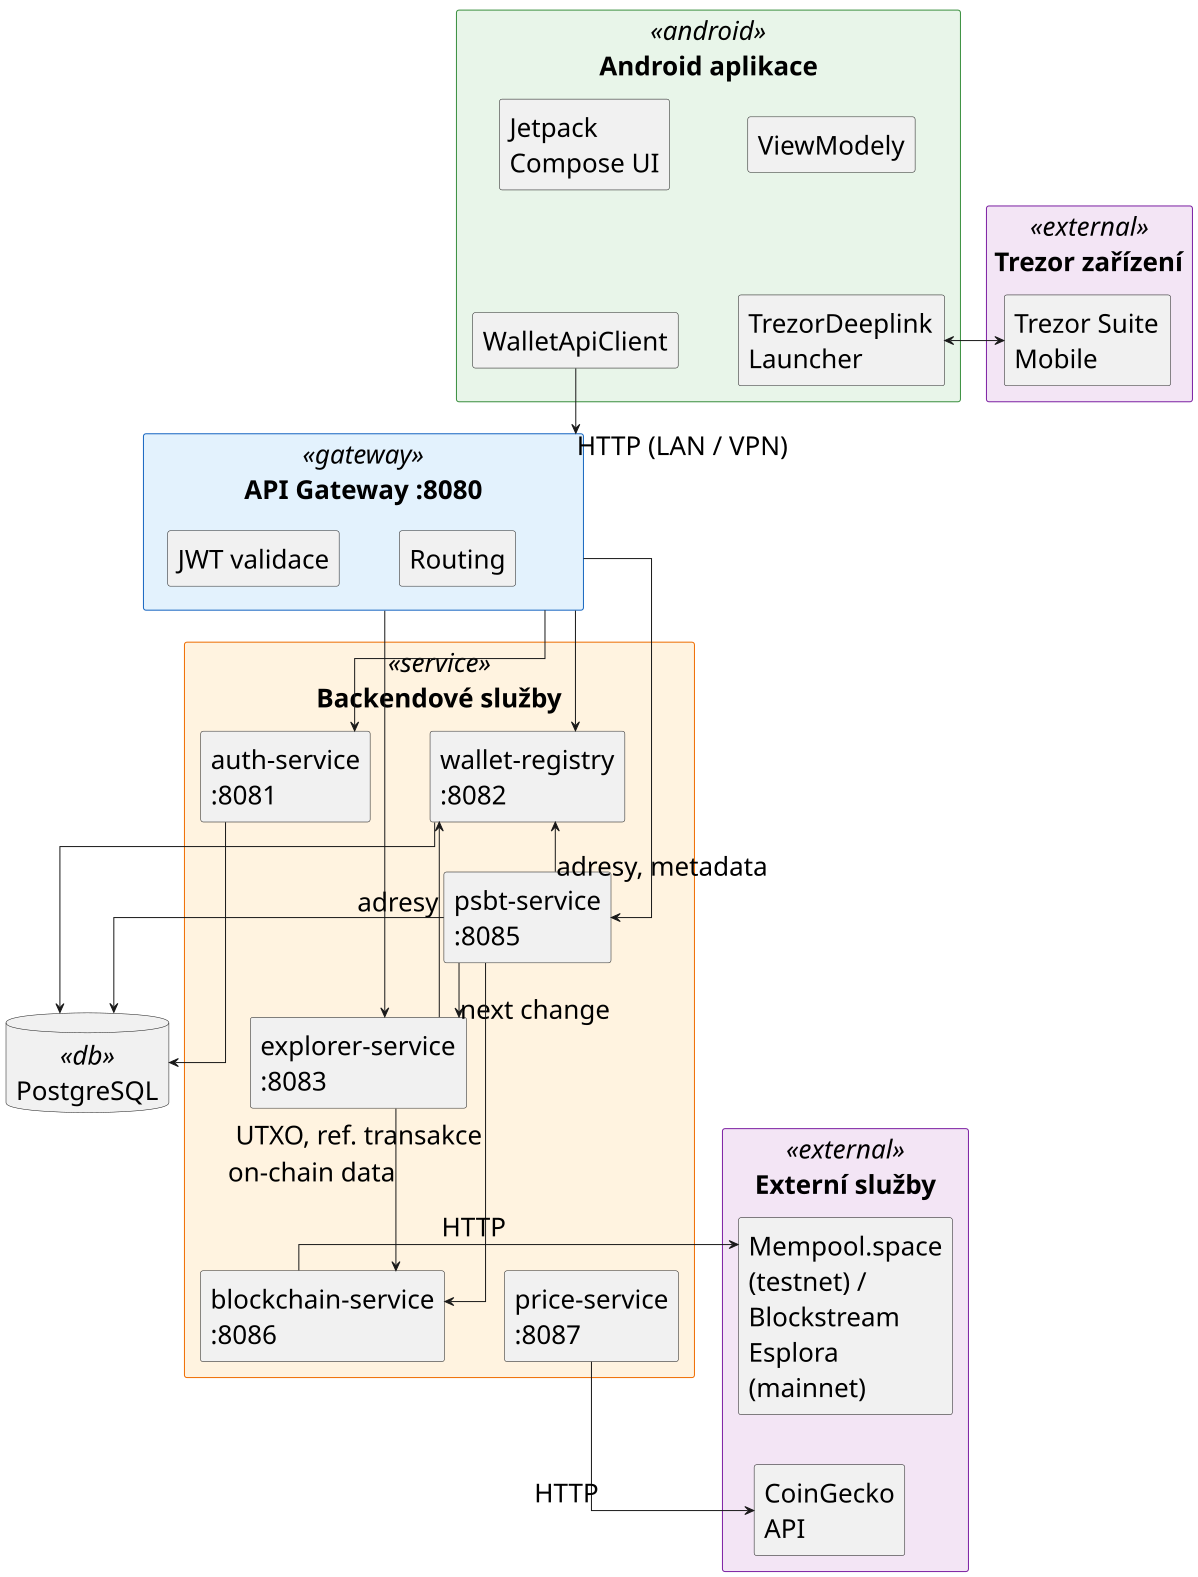
\includegraphics[width=\textwidth]{img/architektura.pdf}
\caption{Schéma architektury systému. Android aplikace komunikuje s~API
Gateway přes HTTP v~izolované LAN či VPN a~s~hardwarovou peněženkou
Trezor přes deeplink protokol zprostředkovaný aplikací Trezor Suite
Mobile. Backendové mikroslužby komunikují mezi sebou interně
a~přistupují k~externím službám (Mempool.space, CoinGecko).}
\label{fig:architektura}
\end{figure}

Při volbě architektonického stylu jsme zvažovali tři varianty:

\begin{description}
\item[Monolitická aplikace] -- jediný nasaditelný artefakt obsahující veškerou
  logiku. Výhodou je jednoduchost vývoje a~nasazení, nevýhodou pak rostoucí
  provázanost kódu a~nemožnost nezávislého škálování jednotlivých komponent.
  Pro peněženku s~vícero jasně oddělitelnými doménami (autentizace, správa peněženek,
  blockchain interakce, PSBT workflow) by monolitický přístup vedl
  k~nepřehledné kódové základně.

\item[Mikroservisy se sdílenou databází] -- služby jsou oddělené, ale sdílejí
  jedno databázové schéma. Tento kompromis usnadňuje dotazy napříč doménami,
  ale zavádí implicitní vazby mezi službami na úrovni datového modelu.
  Změna schématu jedné služby může nechtěně ovlivnit ostatní.

\item[Mikroservisy s~oddělenými databázemi] -- každá služba vlastní svá data
  a~komunikuje s~ostatními výhradně prostřednictvím definovaných API.
  Tento přístup jsme zvolili, protože poskytuje nejsilnější izolaci
  a~umožňuje nezávislý vývoj, nasazení i~škálování jednotlivých služeb.
\end{description}

Zvolili jsme třetí variantu. Systém využívá tři oddělené PostgreSQL~\cite{PostgreSQL} databáze:
jednu pro autentizaci a~správu zařízení (\texttt{auth-service}), jednu pro správu peněženek
a~adres (\texttt{wallet-registry}) a~jednu pro PSBT workflow
(\texttt{psbt-\allowbreak service}). Zbývající služby
(\texttt{explorer-\allowbreak service},
\texttt{blockchain-\allowbreak service},
\texttt{price-\allowbreak service}) jsou bezstavové a~žádnou vlastní
databázi nevyžadují -- slouží jako proxy k~externím API.

\subsection{API Gateway}

API Gateway běží na portu~8080 a~plní několik klíčových rolí:

\begin{itemize}
\item \textbf{Jednotný vstupní bod} -- klientská aplikace komunikuje výhradně
  s~jednou adresou a~nemusí znát topologii backendových služeb.
\item \textbf{Validace JWT tokenů} -- gateway ověřuje platnost přístupových
  tokenů algoritmem RS256 pomocí veřejného klíče získaného z~JWKS endpointu
  \texttt{auth-service}. Požadavky bez platného tokenu jsou odmítnuty
  s~kódem~401, aniž by se dostaly k~cílové službě.
\item \textbf{Směrování požadavků} -- na základě prefixu URL cesty gateway
  přeposílá požadavek na odpovídající mikroslužbu. Například prefix
  \texttt{/api/\allowbreak v1/\allowbreak wallets} je směrován převážně na
  \texttt{wallet-\allowbreak registry} (port~8082), prefix
  \texttt{/api/\allowbreak v1/\allowbreak psbt} na \texttt{psbt-\allowbreak service}
  (port~8085) a~podobně.
\item \textbf{Propagace identity} -- po úspěšné validaci tokenu gateway
  extrahuje identifikátor zařízení (\texttt{device\_id}) a~předává jej
  cílové službě jako query parametr nebo položku v~těle požadavku. Jednotlivé
  služby tak nemusí opakovaně validovat token a~mohou důvěřovat identitě
  předané gateway.
\end{itemize}

Alternativou k~vlastní implementaci gateway by bylo použití existujícího
řešení, například Kong, Traefik či Nginx s~Lua skripty. Zvažovali jsme
především Traefik pro jeho nativní integraci s~Dockerem~\cite{Docker}. Rozhodli jsme se
však pro vlastní implementaci v~Ktoru~\cite{KtorFramework}, protože požadavky na gateway jsou
relativně jednoduché (směrování, JWT validace) a~vlastní řešení umožnilo
sdílet kódovou základnu, datové třídy a~konfiguraci s~ostatními službami
bez nutnosti zavádět další technologii do stacku.

\subsection{Komunikace mezi službami}

Komunikace mezi API Gateway a~mikroslužbami probíhá synchronně prostřednictvím
HTTP požadavků. K~tomuto účelu využíváme Ktor~\cite{KtorFramework} \texttt{HttpClient} s~kotlinovými
korutinami, které zajišťují neblokující I/O operace.

Zvažovali jsme i~asynchronní komunikaci prostřednictvím fronty zpráv
(RabbitMQ, Apache Kafka). Tento přístup by byl vhodný pro systém s~vysokou
zátěží, kde je třeba oddělit producenta a~konzumenta zpráv. V~našem případě
však převažují synchronní operace typu požadavek--odpověď (dotaz na zůstatek,
vytvoření PSBT, podepsání transakce), pro které je HTTP přímočařejší
a~nevyžaduje provoz dalšího infrastrukturního komponentu. Navíc mobilní
klient přirozeně očekává okamžitou odpověď na svůj požadavek.

\subsection{Přehled mikroslužeb}

Systém se skládá z~následujících mikroslužeb:

\begin{description}
\item[\texttt{auth-service} (port 8081)] -- Zajišťuje autentizaci zařízení.
  Při prvním přihlášení vytvoří identitu zařízení na základě fingerprintu
  hardwarové peněženky Trezor a~vydá JWT přístupový token podepsaný algoritmem
  RS256. Token obsahuje \texttt{device\_id} jako \emph{subject} a~má omezenou
  platnost.

\item[\texttt{wallet-registry} (port~8082)] \hfill \\
  Spravuje peněženky, cosignery a~adresy. Pro singlesig peněženky provádí
  derivaci adres podle standardu BIP-32~\cite{BIP32} s~cestou
  \texttt{m/84'/\allowbreak 1'/\allowbreak 0'} (BIP-84~\cite{BIP84}).
  Pro multisig peněženky parsuje output deskriptory ve~formátu
  \texttt{wsh(\allowbreak sorted\-multi(...))} dle BIP-380~\cite{BIP380}
  a~BIP-383~\cite{BIP383} a~provádí derivaci P2WSH adres podle
  BIP-48~\cite{BIP48}.

\item[\texttt{explorer-service} (port 8083)] -- Agreguje data z~blockchainu
  pro konkrétní peněženku. Kombinuje informace o~zůstatku, historii transakcí
  a~nepoužitých výstupech (UTXO) získané z~\texttt{blockchain-service}
  s~adresami z~\texttt{wallet-registry}.

\item[\texttt{psbt-service} (port 8085)] -- Řídí celý životní cyklus PSBT
  transakcí: tvorbu, uložení, podepisování a~broadcast. Při vytváření PSBT
  sestaví parametry potřebné pro podepsání na zařízení Trezor
  prostřednictvím protokolu Trezor Connect~\cite{TrezorConnect}. Dosud
  nepoužitou change adresu pro každou novou transakci si vyžádá
  od~\texttt{explorer-service}; tím je zajištěno, že se~žádná change
  adresa v~čase neopakuje. Pro multisig peněženky sleduje počet
  sebraných podpisů a~umožňuje broadcast po dosažení požadovaného
  prahu~$M$.

\item[\texttt{blockchain-service} (port~8086)] \hfill \\
  Slouží jako proxy k~blockchainovému API. Na mainnetu využívá
  Blockstream Esplora, na testnet4 Mempool.space~\cite{MempoolAPI}
  (obě API sdílejí kompatibilní formát). Poskytuje zůstatky adres,
  seznamy UTXO, detaily transakcí a~aktuální odhady poplatků.

\item[\texttt{price-service} (port 8087)] -- Poskytuje aktuální směnný
  kurz Bitcoinu vůči fiat měnám. Data získává z~CoinGecko
  API~\cite{CoinGeckoAPI} a~kešuje je v~paměti s~krátkou dobou expirace,
  aby se minimalizoval počet externích volání.
\end{description}

%% -----------------------------------------------------------------------
\section{Volba technologií}
\label{sec:technologie}

V~této sekci zdůvodníme volbu konkrétních technologií. U~každé uvádíme, jaké
alternativy jsme zvažovali a~proč jsme se rozhodli právě pro danou variantu.

\subsection{Programovací jazyk: Kotlin}

Pro implementaci celého systému -- jak backendových služeb, tak mobilní
aplikace -- jsme zvolili jazyk Kotlin~\cite{KotlinLang}. Hlavní důvody byly:

\begin{itemize}
\item \textbf{Typová bezpečnost} -- Kotlin je staticky typovaný jazyk
  s~nulovatelností zakódovanou v~typovém systému (\emph{null safety}).
  Pro peněženku manipulující s~finančními prostředky je typová bezpečnost
  obzvláště důležitá, protože zabraňuje celé třídě chyb v~době kompilace.
\item \textbf{Korutiny} -- Kotlinové korutiny poskytují elegantní model
  pro asynchronní programování bez callback hell. Backendové služby zpracovávají
  mnoho souběžných HTTP požadavků a~korutiny umožňují psát neblokující kód
  sekvenčním stylem.
\item \textbf{Sdílený jazyk} -- Použití stejného jazyka pro backend i~frontend
  umožňuje sdílet datové třídy, validační logiku a~mentální model mezi oběma
  částmi systému. Vývojář nepotřebuje přepínat mezi různými jazyky a~jejich
  idiomy.
\item \textbf{Oficiální jazyk pro Android} -- Google označuje Kotlin jako
  preferovaný jazyk pro vývoj Android aplikací, což zaručuje dlouhodobou
  podporu a~rozsáhlý ekosystém knihoven.
\end{itemize}

Zvažovali jsme rovněž jazyk Dart (s~frameworkem Flutter) pro mobilní aplikaci
a~Go nebo TypeScript pro backend. Dart by umožnil multiplatformní vývoj
(Android i~iOS), avšak za cenu ztráty sdíleného jazyka s~backendem.
Bitcoinové knihovny pro Dart sice existují (např.\ \texttt{bitcoin\_flutter},
\texttt{dartsv}), ale jde o~menší komunitní projekty s~méně zralým ekosystémem
než JVM platforma s~knihovnou bitcoinj~\cite{BitcoinJ}. Go nabízí výborný výkon
a~jednoduchost a~disponuje kvalitními Bitcoinovými knihovnami (např.\ \texttt{btcd}),
ale postrádá vestavěnou podporu pro Android vývoj -- mobilní aplikaci
by bylo nutné řešit samostatně v~jiném jazyce, čímž by se ztratila výhoda
sdíleného kódu.

\subsection{Backend framework: Ktor}

\begin{sloppypar}
Pro implementaci backendových služeb jsme zvolili framework
Ktor \cite{KtorFramework}. Alternativou byl především Spring Boot,
nejpoužívanější framework pro JVM back\-endy. Ktor jsme upřednostnili
z~následujících důvodů:
\end{sloppypar}

\begin{itemize}
\item \textbf{Nativní podpora korutin} -- Ktor je od základu navržen
  s~kotlinovými korutinami. Každý příchozí požadavek je zpracován v~korutině,
  což umožňuje neblokující obsluhu tisíců souběžných spojení s~minimální
  paměťovou náročností.
\item \textbf{Minimalistický design} -- Ktor nepřidává žádnou \uv{magii} --
  nepoužívá reflexi, anotační procesory ani dependency injection kontejner.
  Konfigurace probíhá explicitně v~kódu, což zvyšuje čitelnost
  a~předvídatelnost chování.
\item \textbf{Modulární architektura} -- Funkcionalita se přidává formou
  pluginů (autentizace, serializace, CORS, logování). Výsledný artefakt
  obsahuje pouze skutečně používané komponenty.
\item \textbf{Nízká paměťová náročnost} -- Mikroslužby nasazujeme v~Docker
  kontejnerech a~pro provoz peněženky s~řádově jednotkami až desítkami
  uživatelů nepotřebujeme těžký aplikační framework. Ktor služba startuje
  v~řádu stovek milisekund a~spotřebuje výrazně méně paměti než srovnatelná
  Spring Boot aplikace.
\end{itemize}

Spring Boot by nabídl robustnější ekosystém (Spring Security, Spring Data),
ale pro naše účely by představoval zbytečnou složitost. Naše služby mají
úzce vymezené API s~řádově jednotkami endpointů a~nepotřebují pokročilé
funkce jako ORM nebo deklarativní security pravidla.

\subsection{Mobilní framework: Jetpack Compose}

\begin{sloppypar}
Pro uživatelské rozhraní mobilní aplikace jsme zvolili Jetpack
Compose \cite{JetpackCompose}, moderní deklarativní UI toolkit
od~Googlu. Alternativou byl klasický přístup pomocí XML layout
souborů a~View systému.
\end{sloppypar}

Jetpack Compose jsme zvolili z~následujících důvodů:

\begin{itemize}
\item \textbf{Deklarativní paradigma} -- UI se popisuje jako funkce stavu.
  Při změně stavu se automaticky překreslí pouze dotčené části, bez nutnosti
  manuální manipulace s~View objekty. To vede k~méně chybovému a~lépe
  testovatelnému kódu.
\item \textbf{Méně boilerplate kódu} -- Odpadá nutnost definovat
  XML layouty, View\-Holdery, Adaptery a~další ceremoniální kód
  typický pro starší Android přístup. UI komponenty se píší přímo
  v~Kotlinu.
\item \textbf{Budoucí standard} -- Google aktivně doporučuje Jetpack Compose
  jako preferovaný způsob tvorby Android UI a~investuje do jeho rozvoje.
  Nové Android API se primárně navrhují s~ohledem na Compose.
\item \textbf{Integrace s~Kotlinem} -- Compose přirozeně využívá Kotlinové
  jazykové konstrukce (lambda výrazy, extension funkce, korutiny), což vede
  ke konzistentnímu a~idiomatickému kódu.
\end{itemize}

\subsection{Databáze: PostgreSQL}

Jako databázový systém jsme zvolili PostgreSQL~\cite{PostgreSQL}. Zvažovali
jsme rovněž SQLite (vestavěnou přímo v~mobilní aplikaci) a~MySQL/MariaDB.

PostgreSQL jsme upřednostnili z~následujících důvodů:

\begin{itemize}
\item \textbf{Silná konzistence a~ACID} -- Pro systém pracující s~finančními
  transakcemi je zásadní, aby databázové operace byly atomické a~konzistentní.
  Například při ukládání podpisu k~PSBT je nutné atomicky inkrementovat
  počítadlo podpisů a~ověřit dosažení prahu.
\item \textbf{Souběžné zápisy z~více služeb} -- v~mikroservisní architektuře
  do téže databáze paralelně píše více služeb i~několik instancí téže
  služby. Postgres MVCC zajišťuje korektní izolaci souběžných transakcí
  bez nutnosti aplikačního zamykání.
\item \textbf{Zralost a~rozšířenost} -- PostgreSQL je jeden z~nejrozšířenějších
  open-source databázových systémů s~rozsáhlou dokumentací a~komunitou.
\end{itemize}

SQLite by bylo vhodné řešení pro čistě mobilní aplikaci bez backendu, ale
v~zvolené architektuře databáze běží na serveru a~je sdílena mezi požadavky
od různých zařízení. MySQL by bylo funkčně rovnocenné pro většinu operací;
PostgreSQL jsme upřednostnili pro robustnější MVCC izolaci souběžných
transakcí a~širší ekosystém nástrojů (Flyway migrace, Exposed ORM).

\subsection{Kontejnerizace: Docker Compose}

Pro nasazení a~orchestraci všech backendových služeb používáme Docker
Compose~\cite{Docker}. Každá mikroslužba, API Gateway a~databázové instance
běží ve vlastním kontejneru. Zvažovali jsme i~Kubernetes, který by umožnil
pokročilé škálování a~self-healing, ale pro vývoj a~provoz peněženky
s~omezeným počtem uživatelů je Kubernetes zbytečně komplexní. Docker Compose
plně postačuje a~umožňuje jedním příkazem (\texttt{docker compose up})
spustit celý systém včetně databází, migrací a~všech služeb.

Hlavní výhody kontejnerizace v~kontextu tohoto systému:

\begin{itemize}
\item \textbf{Reprodukovatelné prostředí} -- vývojové, testovací a~produkční
  prostředí je identické, čímž se eliminují problémy typu \uv{u~mě to funguje}.
\item \textbf{Izolace služeb} -- každá služba běží ve vlastním kontejneru
  se svými závislostmi. Aktualizace jedné služby neovlivní ostatní.
\item \textbf{Definovaná síťová topologie} -- Docker Compose vytváří interní
  síť, kde se služby navzájem adresují jménem kontejneru. Mobilní aplikace
  komunikuje pouze s~gateway, ostatní služby nejsou z~vnějšku dostupné.
\end{itemize}

\subsection{Blockchainové API}

Pro získávání dat z~Bitcoin blockchainu (zůstatky adres, seznamy UTXO,
detaily transakcí, odhady poplatků) jsme zvažovali tři varianty:

\begin{itemize}
\item \textbf{Vlastní Bitcoin full node} -- poskytuje maximální nezávislost
  a~soukromí, ale vyžaduje stovky gigabajtů diskového prostoru a~kontinuální
  synchronizaci s~sítí. Pro testovací a~vývojové účely je toto nepraktické.
\item \textbf{Blockstream Esplora API}~\cite{BlockstreamEsplora} -- open-source
  řešení s~veřejným REST API a~tolerantními rate limity. Nepodporuje však síť testnet4
  (novější testovací síť Bitcoinu), která je potřebná pro vývoj.
\item \textbf{Mempool.space API} -- rovněž open-source, s~plnou podporou
  testnet4, bez nutnosti API klíče. Poskytuje kvalitní odhady poplatků
  na základě aktuálního stavu mempoolu. Oproti Blockstream Esplora má
  však přísnější rate limity.
\end{itemize}

Obě služby (Blockstream Esplora i~Mempool.space) sdílejí kompatibilní
REST API formát, což umožňuje použít stejnou klientskou implementaci
pro obě. Využíváme proto obě: na mainnetu Blockstream Esplora~\cite{BlockstreamEsplora}
(\url{https://blockstream.info/api}) pro jeho stabilitu a~tolerantní
rate limity, na testnet4 Mempool.space
(\url{https://mempool.space/testnet4/api}), protože Blockstream Esplora
testnet4 nepodporuje. Aktivní poskytovatel se volí podle konfigurace sítě.

Díky izolaci blockchainové komunikace do samostatné služby
\texttt{blockchain-\allowbreak service} je možné poskytovatele snadno
zaměnit nebo přidat podporu vlastního full node bez zásahu do zbytku systému.

\subsection{Cenový zdroj: CoinGecko API}

Pro zobrazení aktuální hodnoty prostředků ve fiat měně používáme
CoinGecko API~\cite{CoinGeckoAPI}. CoinGecko nabízí bezplatný tier
s~dostatečným limitem požadavků (30~volání za minutu na Demo API
klíči), podporuje desítky fiat měn a~vyžaduje pouze bezplatnou
registraci. Alternativou by bylo CoinMarketCap API, které pro
bezplatný plán nabízí méně velkorysé limity.

%% -----------------------------------------------------------------------
\section{Bezpečnostní model}
\label{sec:bezpecnost}

Bezpečnostní model aplikace je postaven na fundamentálním principu:
\textbf{server nikdy nedisponuje privátními klíči uživatele}. Veškeré
kryptografické operace spojené s~podepisováním transakcí probíhají výhradně
na hardwarovém zařízení Trezor, které nikdy neopustí fyzický dosah uživatele.
I~v~případě kompletní kompromitace serveru tak útočník nezíská prostředky
k~odcizení Bitcoinů.

\subsection{Autentizace a identita}

Pro autentizaci zařízení používáme JWT (\emph{JSON Web Token}) tokeny
podepsané asymetrickým algoritmem RS256. Schéma autentizace funguje
následovně:

\begin{enumerate}
\item Uživatel připojí hardwarovou peněženku Trezor k~mobilnímu zařízení.
\item Aplikace prostřednictvím Trezor Connect získá veřejné informace
  o~zařízení -- především \emph{fingerprint} kořenového veřejného klíče.
\item Z~fingerprintu je deterministicky odvozen \texttt{device\_id}
  (UUID verze~3 s~prefixem \texttt{trezor:}).
\item \texttt{auth-service} uloží identitu zařízení a~vydá JWT token
  podepsaný svým privátním RSA klíčem. Token obsahuje \texttt{device\_id}
  jako \emph{subject} a~má omezenou dobu platnosti.
\item API Gateway validuje token při každém požadavku pomocí veřejného
  klíče získaného z~JWKS endpointu \texttt{auth-service}.
\end{enumerate}

Celý průběh autentizace zachycuje obrázek~\ref{fig:auth-flow}.

\begin{figure}[htbp]
\centering
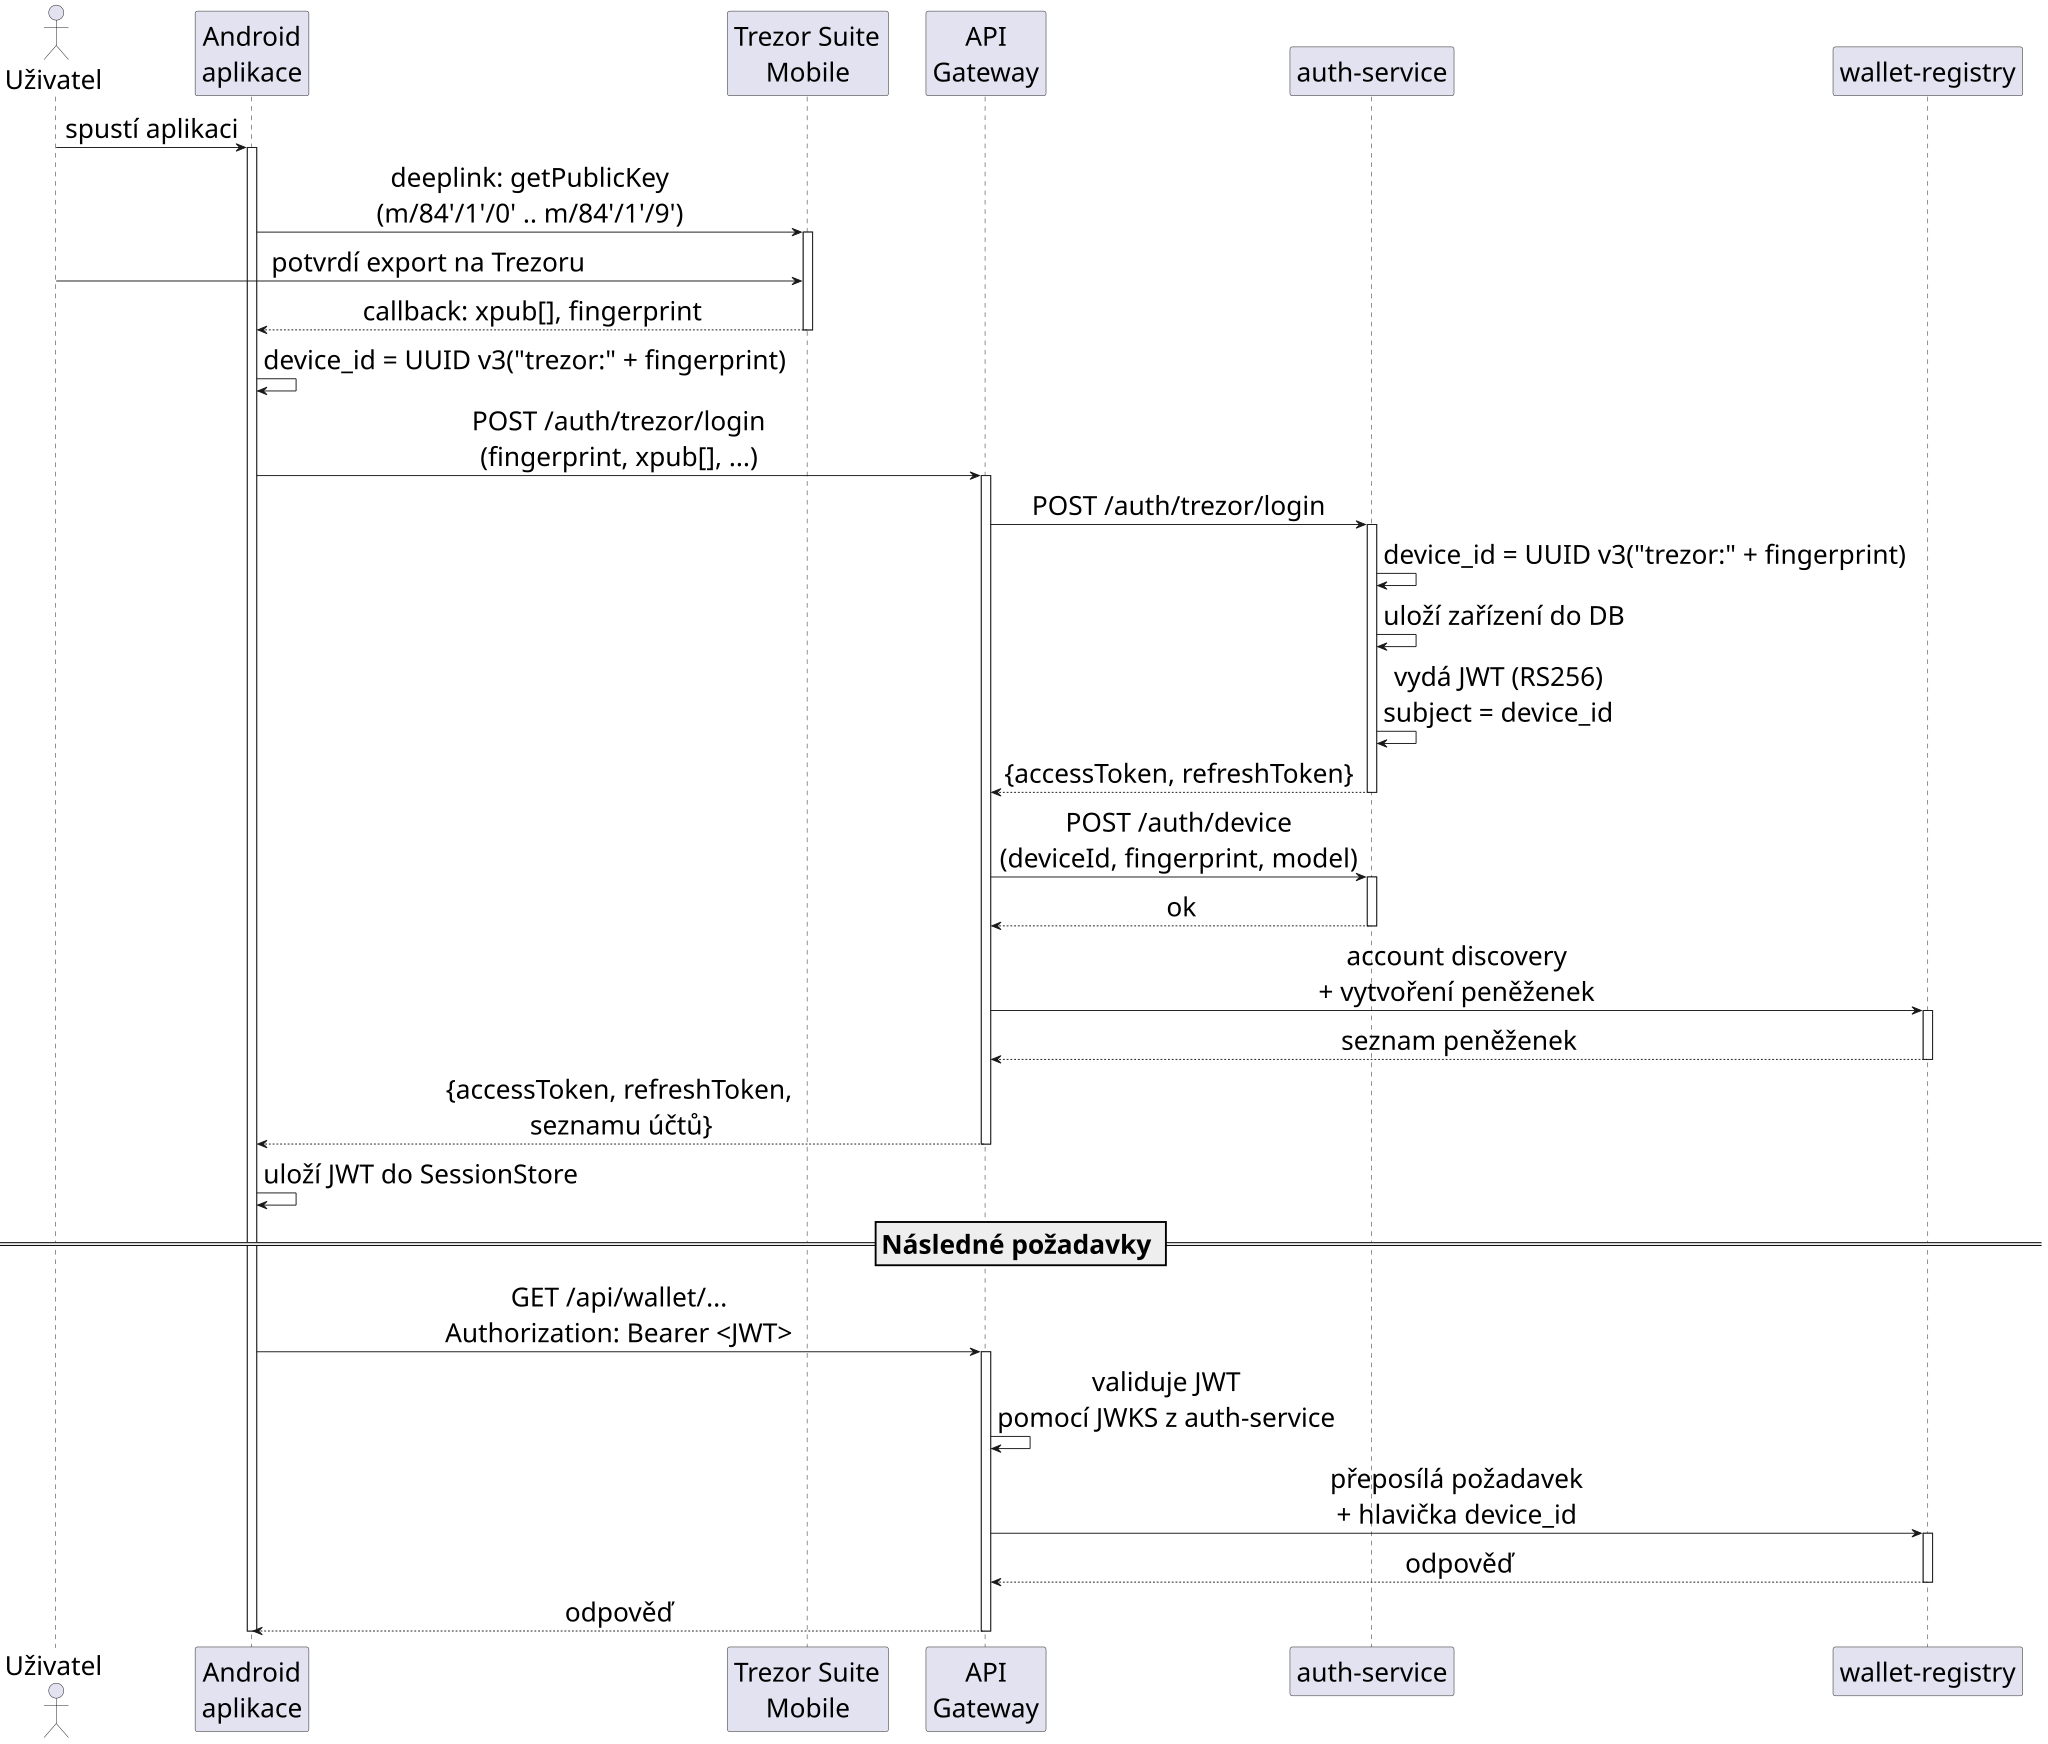
\includegraphics[width=\textwidth,height=0.85\textheight,keepaspectratio]{img/auth-flow.pdf}
\caption{Sekvenční diagram autentizace. Uživatel exportuje veřejné klíče
z~Trezoru přes Trezor Suite Mobile, \texttt{auth-service} uloží zařízení
a~vydá JWT token, API Gateway následně validuje token při každém požadavku.}
\label{fig:auth-flow}
\end{figure}

Zvažovali jsme i~jednodušší autentizační schémata -- například symetrické
HMAC tokeny nebo statické API klíče. Asymetrický RS256 jsme zvolili proto,
že umožňuje distribuci veřejného klíče přes JWKS endpoint: gateway i~ostatní
služby mohou nezávisle ověřovat tokeny, aniž by sdílely tajný klíč
s~\texttt{auth-service}. To snižuje plochu útoku -- kompromitace gateway
neumožní vystavovat falešné tokeny.

Identita zařízení je odvozena z~fingerprintu Trezoru, nikoliv z~uživatelského
jména a~hesla. Tento přístup reflektuje specifika aplikace: uživatel
se neidentifikuje svou osobou, ale svým hardwarovým zařízením. Zároveň
tak odpadá nutnost spravovat hesla, řešit jejich reset a~chránit je
před únikem.

\subsubsection{Obnova přístupového tokenu přes refresh token}
\label{subsec:refresh-token}

Přístupový JWT token má platnost 24~hodin. Bez dalšího mechanismu by
uživatel musel po~každém vypršení znovu exportovat veřejné klíče
z~Trezoru, což by výrazně zhoršilo uživatelský komfort -- uživatel
by přitom neměnil identitu, pouze obnovoval relaci. Proto \texttt{auth-service}
při~přihlášení vydá vedle přístupového tokenu ještě tzv.~\emph{refresh
token} s~delší platností (30~dní), který aplikace uchová spolu
s~přístupovým tokenem a~použije jej k~obnově, jakmile přístupový token
vyprší.

Refresh tokeny jsou navrženy jako \emph{jednorázové} -- každý token
lze použít pouze k~jediné výměně za~novou dvojici. Rotace probíhá takto:

\begin{enumerate}
\item Aplikace pošle aktuální refresh token na \texttt{POST /auth/token/refresh}.
\item \texttt{auth-service} v~jedné databázové transakci vyhledá záznam
  podle hashe tokenu, ověří, že není expirovaný ani dříve revokovaný,
  atomicky nastaví sloupec \texttt{revoked\_at} a~vydá novou dvojici
  (přístupový $+$ refresh token).
\item Aplikace nové tokeny uloží do~perzistence a~starý refresh token
  už znovu nepoužije.
\end{enumerate}

Krok~2 je race-safe: klauzule \texttt{UPDATE \ldots WHERE revoked\_at
IS NULL} zajišťuje, že pokud stejný refresh token dorazí na~server
souběžně dvakrát, vyhraje pouze jeden \texttt{UPDATE}; druhý uvidí
nulový počet aktualizovaných řádků a~vrátí klientovi~401. Tím se brání
situaci, kdy by dvě souběžné výměny vygenerovaly dva platné refresh
tokeny ze~stejného originálu.

V~databázi je uložen pouze SHA-256 hash tokenu, nikoli jeho otevřená
hodnota. Případný únik obsahu tabulky \texttt{refresh\_tokens} tedy
neumožní útočníkovi používat aktivní tokeny -- získá pouze otisky,
ze~kterých původní hodnotu nelze zpětně odvodit. Otevřená hodnota
existuje výhradně v~paměti klienta a~v~jeho lokálním perzistentním
úložišti.

\subsection{Absence privátních klíčů na serveru}

Na serveru nejsou uloženy žádné privátní klíče, seed fráze ani jakékoliv
materiály, z~nichž by bylo možné privátní klíče odvodit. Server disponuje
pouze veřejnými klíči (xpub) potřebnými pro derivaci adres a~ověřování
podpisů. Toto oddělení je zásadní pro bezpečnostní model aplikace --
i~v~případě úplné kompromitace serveru útočník získá pouze veřejné informace
(adresy, zůstatky, historii transakcí), nikoliv prostředky k~odcizení
prostředků.

\subsection{Podepisování transakcí přes Trezor Connect}
\label{subsec:trezor-connect}

Jak jsme analyzovali v~sekci~\ref{sec:analyza-trezor}, podepisování
transakcí probíhá prostřednictvím deeplink protokolu Trezor
Connect~\cite{TrezorConnect} s~aplikací Trezor Suite Mobile jako
prostředníkem. Konkrétní průběh podepisování:

\begin{enumerate}
\item Backend (\texttt{psbt-service}) sestaví z~PSBT transakce parametry
  ve formátu požadovaném Trezor Connect (vstupy s~derivačními cestami,
  výstupy s~adresami a~částkami).
\item Mobilní aplikace obdrží tyto parametry a~otevře Trezor Suite Mobile
  prostřednictvím deeplinku Trezor Connect
  (\texttt{https://\allowbreak connect.\allowbreak trezor.\allowbreak io/\allowbreak 9/\allowbreak deeplink/\allowbreak 1/}).
\item Uživatel ověří detaily transakce na displeji hardwarové peněženky
  a~potvrdí podpis fyzickým stisknutím tlačítka.
\item Trezor Suite Mobile vrátí výsledek zpět do aplikace prostřednictvím
  callback deeplinku.
\item Trezor Connect vždy vrací jak \texttt{serializedTx}, tak pole
  \texttt{signatures}. V~případě singlesig peněženky aplikace použije
  serializovanou transakci přímo k~broadcastu. V~případě multisig peněženky
  aplikace extrahuje pole podpisů a~odešle je na backend, který je přidá
  k~PSBT a~zkontroluje, zda byl dosažen požadovaný práh~$M$.
\end{enumerate}

Tento mechanismus zajišťuje, že privátní klíč nikdy neopustí bezpečné
prostředí hardwarové peněženky. Uživatel má plnou kontrolu nad tím, jaké
transakce podepisuje, protože detaily vždy ověřuje přímo na zařízení Trezor.

Kromě podepisování transakcí využíváme Trezor Connect i~pro \textbf{ověření
přijímací adresy na zařízení}. Při příjmu prostředků může uživatel stisknout
tlačítko \emph{Zobrazit na Trezoru}, čímž aplikace prostřednictvím deeplinku
zavolá metodu \texttt{getAddress} s~parametrem \texttt{showOnTrezor: true}.
Trezor na svém displeji zobrazí adresu odvozenou přímo z~klíčů uložených
v~zařízení a~uživatel ji může vizuálně porovnat s~adresou zobrazenou
v~aplikaci. Tím se eliminuje riziko, že by kompromitovaná aplikace nebo
server podvrhly cizí adresu -- útočník by musel současně ovládnout
i~firmware hardwarové peněženky, což je prakticky nemožné. Pro multisig
peněženky parametry volání zahrnují veřejné klíče všech cosignerů seřazené
podle BIP-67~\cite{BIP67}, aby Trezor mohl nezávisle odvodit správnou
P2WSH adresu.

Celý průběh podepisování zachycují obrázky~\ref{fig:trezor-signing-1}
a~\ref{fig:trezor-signing-2}.

\begin{figure}[htbp]
\centering
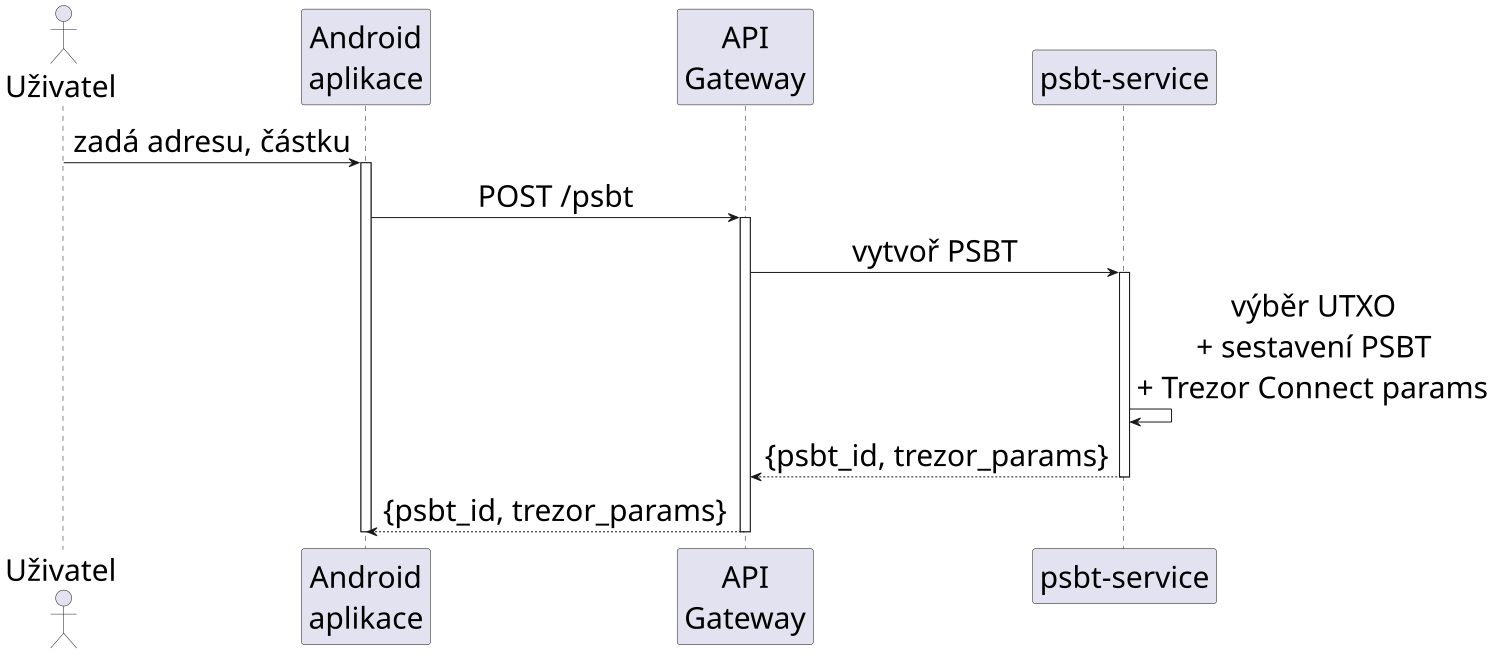
\includegraphics[width=\textwidth]{img/trezor-signing-1.pdf}
\caption{Sekvenční diagram podepisování -- první část: vytvoření PSBT na
backendu. Aplikace zadá požadavek API Gateway, \texttt{psbt-service}
vybere UTXO, sestaví PSBT a~připraví parametry pro Trezor Connect.}
\label{fig:trezor-signing-1}
\end{figure}

V~první fázi backend sestaví částečně podepsanou transakci ve~formátu
BIP-174. Pro multisig peněženku PSBT obsahuje kromě nepodepsané
transakce i~kompletní witness skript, derivační cesty všech cosignerů
a~předchozí transakce referencovaných UTXO -- vše, co Trezor potřebuje
k~ověření před podpisem. Spolu s~PSBT backend vrací strukturovaný
JSON objekt s~parametry pro Trezor Connect, který přesně odpovídá
formátu očekávanému metodou \texttt{signTransaction}.

V~druhé fázi mobilní aplikace předá tyto parametry Trezor Suite Mobile
a~uživatel transakci podepíše na hardwarovém zařízení. Návrat do aplikace
se liší podle typu peněženky: pro singlesig Trezor vrátí kompletní
serializovanou transakci, kterou aplikace pošle k~broadcastu; pro multisig
vrací pouze pole podpisů, které backend přidá do PSBT na pozici
odpovídající aktuálnímu cosignerovi.

\begin{figure}[htbp]
\centering
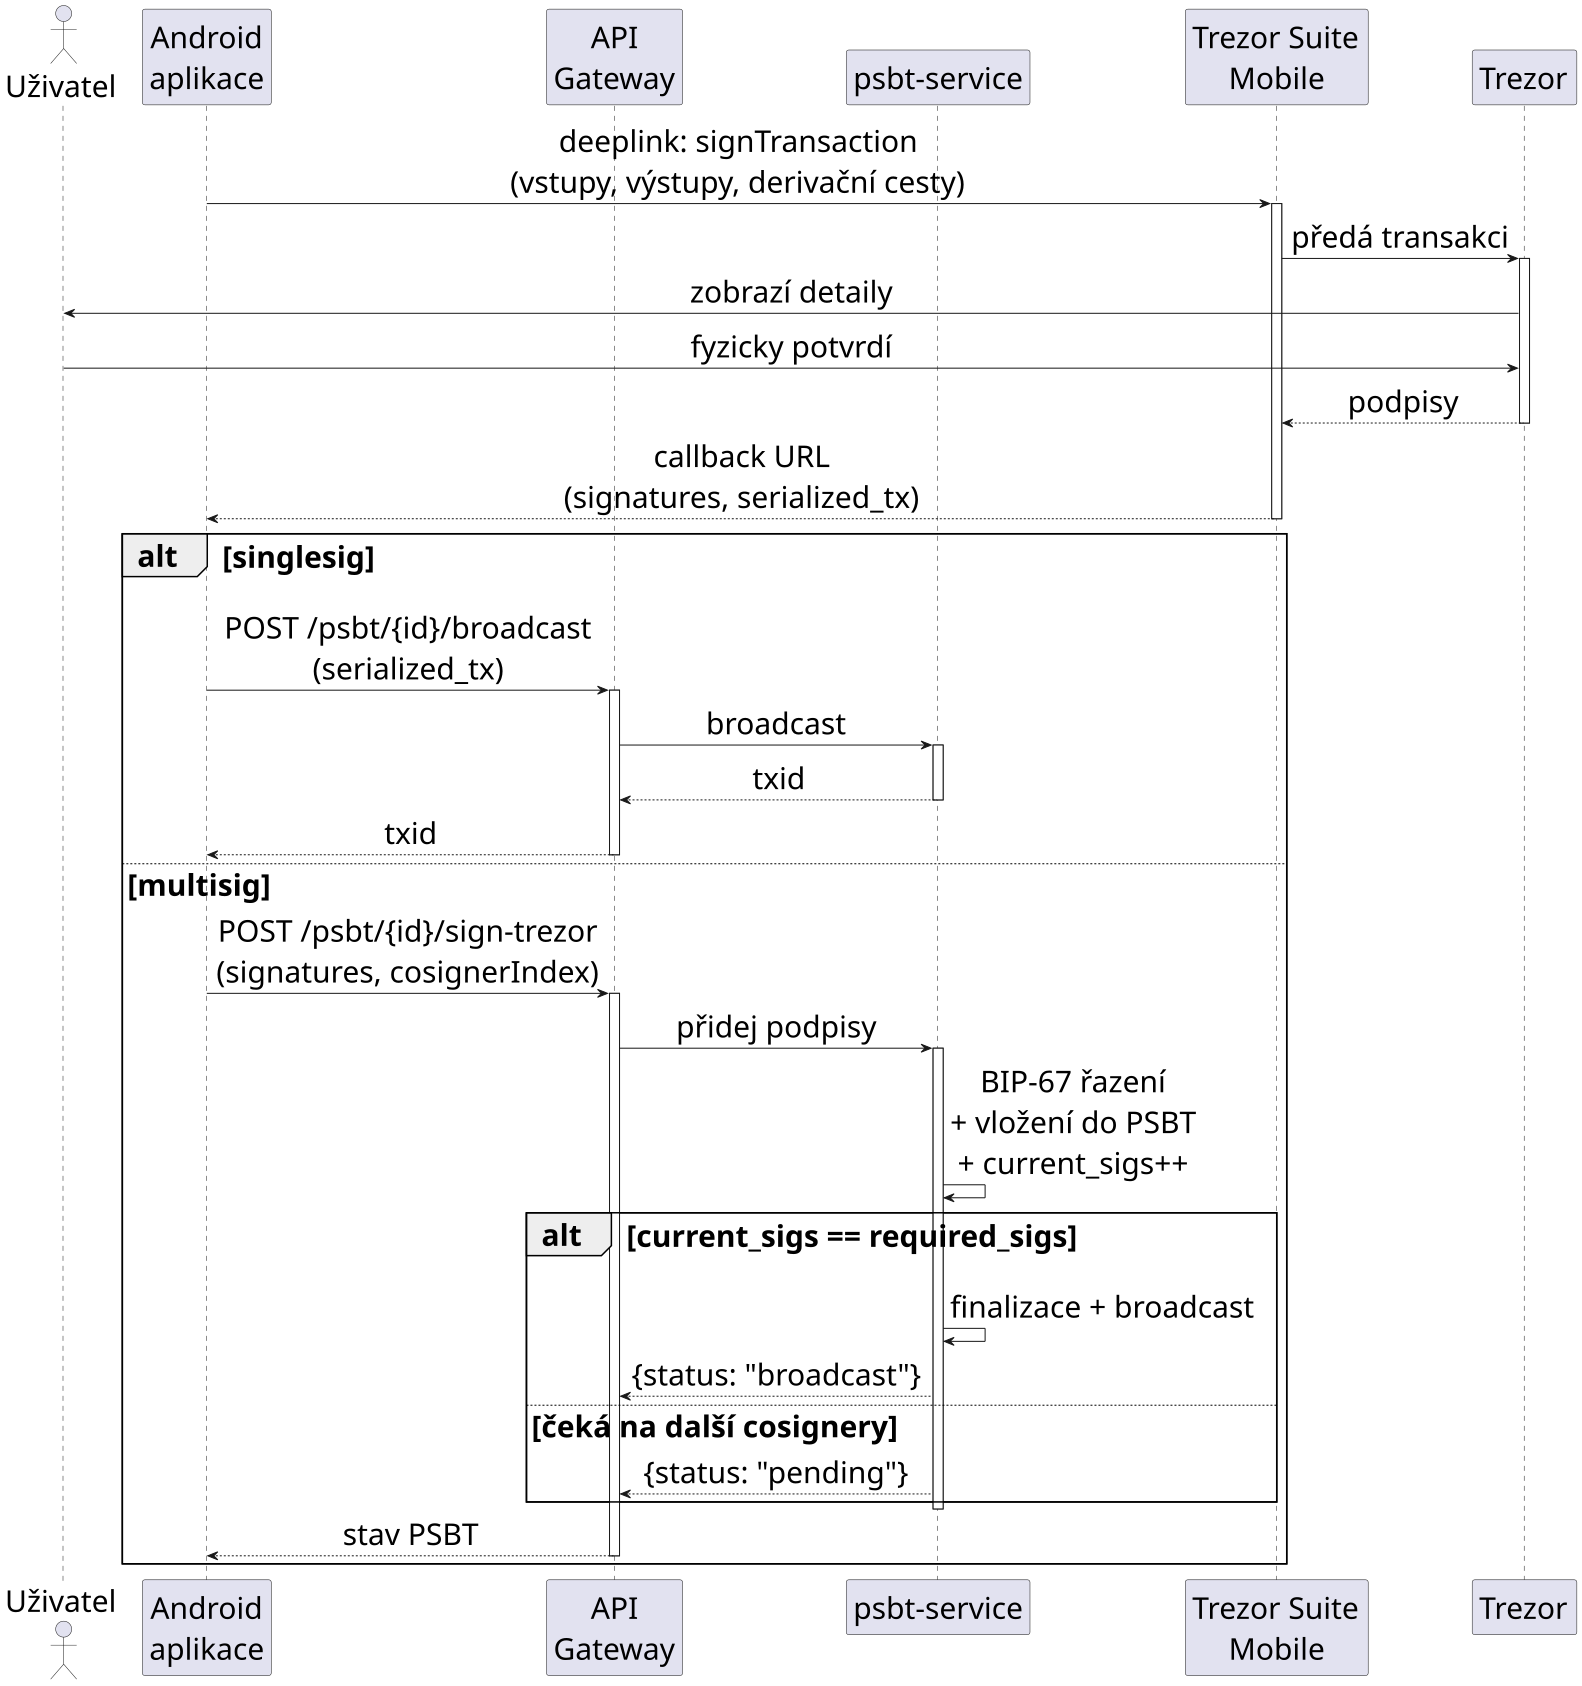
\includegraphics[width=\textwidth]{img/trezor-signing-2.pdf}
\caption{Sekvenční diagram podepisování -- druhá část: podpis na hardwarovém
zařízení a~následný broadcast (singlesig) nebo přidání dílčího podpisu
(multisig). Detaily transakce uživatel vždy ověřuje přímo na displeji
Trezoru.}
\label{fig:trezor-signing-2}
\end{figure}

%% -----------------------------------------------------------------------
\section{Datový model}
\label{sec:datovy-model}

Datový model systému je rozdělen do tří databází odpovídajících mikroslužbám,
které potřebují perzistentní úložiště. V~této sekci popíšeme hlavní entity
a~jejich vztahy.

\subsection{Databáze autentizační služby}

Databáze \texttt{auth-service} obsahuje dvě tabulky:

\begin{description}
\item[\texttt{devices}] -- Uchovává identitu autentizovaných zařízení.
  Primárním klíčem je \texttt{device\_id} (UUID odvozený z~fingerprintu).
  Dále obsahuje \texttt{fingerprint} kořenového veřejného klíče Trezoru,
  \texttt{model} (typ zařízení) a~\texttt{label} (uživatelský název).

\item[\texttt{refresh\_tokens}] -- Persistentní úložiště refresh tokenů
  s~jednorázovou rotací. Primárním klíčem je SHA-256 hash tokenu
  (otevřená hodnota se v~databázi nikdy neukládá, viz
  sekci~\ref{subsec:refresh-token}). Dále obsahuje
  \texttt{device\_\allowbreak id} (zařízení, kterému token patří),
  \texttt{fingerprint} kořenového klíče,
  \texttt{expires\_\allowbreak at} (platnost, default 30~dní),
  \texttt{created\_\allowbreak at} (vystavení) a~\texttt{revoked\_\allowbreak at}
  (čas revokace, \texttt{NULL} značí dosud platný token). Sloupec
  \texttt{revoked\_\allowbreak at} je load-bearing pro race-safe rotaci
  popsanou v~sekci~\ref{subsec:refresh-token}.
\end{description}

\subsection{Databáze wallet-registry}

Databáze \texttt{wallet-registry} obsahuje entity pro správu peněženek,
cosignerů a~adres:

\begin{description}
\item[\texttt{wallets}] {\sloppy -- Reprezentuje peněženku
  (singlesig nebo multisig). Identifikátor
  \texttt{wallet\_\allowbreak id} je deterministicky generován:
  u~multisig peněženek jako zkrácený SHA-256 hash output deskriptoru
  (s~prefixem sítě), u~singlesig jako kompozitní klíč
  \texttt{wallet-\{fingerprint\}-\{network\}-\{scriptType\}-\{accountIndex\}}.
  Oba přístupy zajišťují, že totožná peněženka vždy vede ke~stejnému
  identifikátoru. Tabulka dále obsahuje
  \texttt{network} (mainnet/\allowbreak testnet),
  \texttt{type} (SINGLE\_\allowbreak SIG~/~MULTI\_\allowbreak SIG),
  \texttt{script\_\allowbreak type} (P2WPKH~/~P2WSH), požadovaný
  počet podpisů~$M$, celkový počet cosignerů~$N$ a~dva kompletní
  deskriptory (\texttt{receive\_\allowbreak descriptor} pro přijímací
  adresy a~\texttt{change\_\allowbreak descriptor} pro change
  adresy).\par}

\item[\texttt{cosigners}] -- Uchovává veřejné klíče (xpub) jednotlivých
  cosignerů. Každý záznam obsahuje \texttt{fingerprint} nadřazeného klíče,
  \texttt{origin\_path} (derivační cesta, například \texttt{48'/1'/0'/2'})
  a~samotný rozšířený veřejný klíč \texttt{xpub}.

\item[\texttt{wallet\_cosigners}] -- Vazební tabulka propojující peněženky
  s~cosignery. Obsahuje \texttt{cosigner\_index}, který určuje pozici
  cosignera v~rámci peněženky. Tento index je důležitý pro správné řazení
  veřejných klíčů podle standardu BIP-67~\cite{BIP67} při sestavování
  multisig skriptů.

\item[\texttt{wallet\_members}] -- Propojuje zařízení s~peněženkami.
  Umožňuje jednomu zařízení být členem více peněženek a~jedné peněžence
  mít více členských zařízení. Obsahuje \texttt{account\_index}, který
  identifikuje, kterým cosignerem dané zařízení v~rámci peněženky je.

\item[\texttt{wallet\_addresses}] -- Ukládá předem derivované adresy pro každou
  peněženku. Každá adresa má \texttt{address\_type} (receive/change),
  \texttt{address\_index} (pořadí v~derivační cestě) a~samotnou adresu ve formátu
  Bech32 (\texttt{tb1q...} pro testnet, \texttt{bc1q...} pro mainnet).
  Oba typy výstupů (P2WPKH i~P2WSH) sdílejí prefix \texttt{bc1q}/\texttt{tb1q},
  liší se pouze délkou adresy. Předderivování adres umožňuje rychlou odpověď na dotazy
  bez nutnosti opakované derivace.

\item[\texttt{cosigner\_labels}] -- Ukládá uživatelská pojmenování
  cosignerů v~rámci konkrétní multisig peněženky (například
  \uv{Alicin klíč}, \uv{Pepa}). Záznam je vázán na trojici
  (\texttt{wallet\_\allowbreak id}, \texttt{cosigner\_\allowbreak index},
  \texttt{device\_\allowbreak id}), takže název je privátní pro dané
  zařízení a~ostatním cosignerům se nezobrazuje. Důvodem je ochrana
  soukromí: osobní poznámky o~spolupodepisovatelích by neměly prosakovat
  mezi členy sdílené peněženky.
\end{description}

Schéma vztahů mezi entitami zachycuje obrázek~\ref{fig:er-diagram}.

\begin{figure}[htbp]
\centering
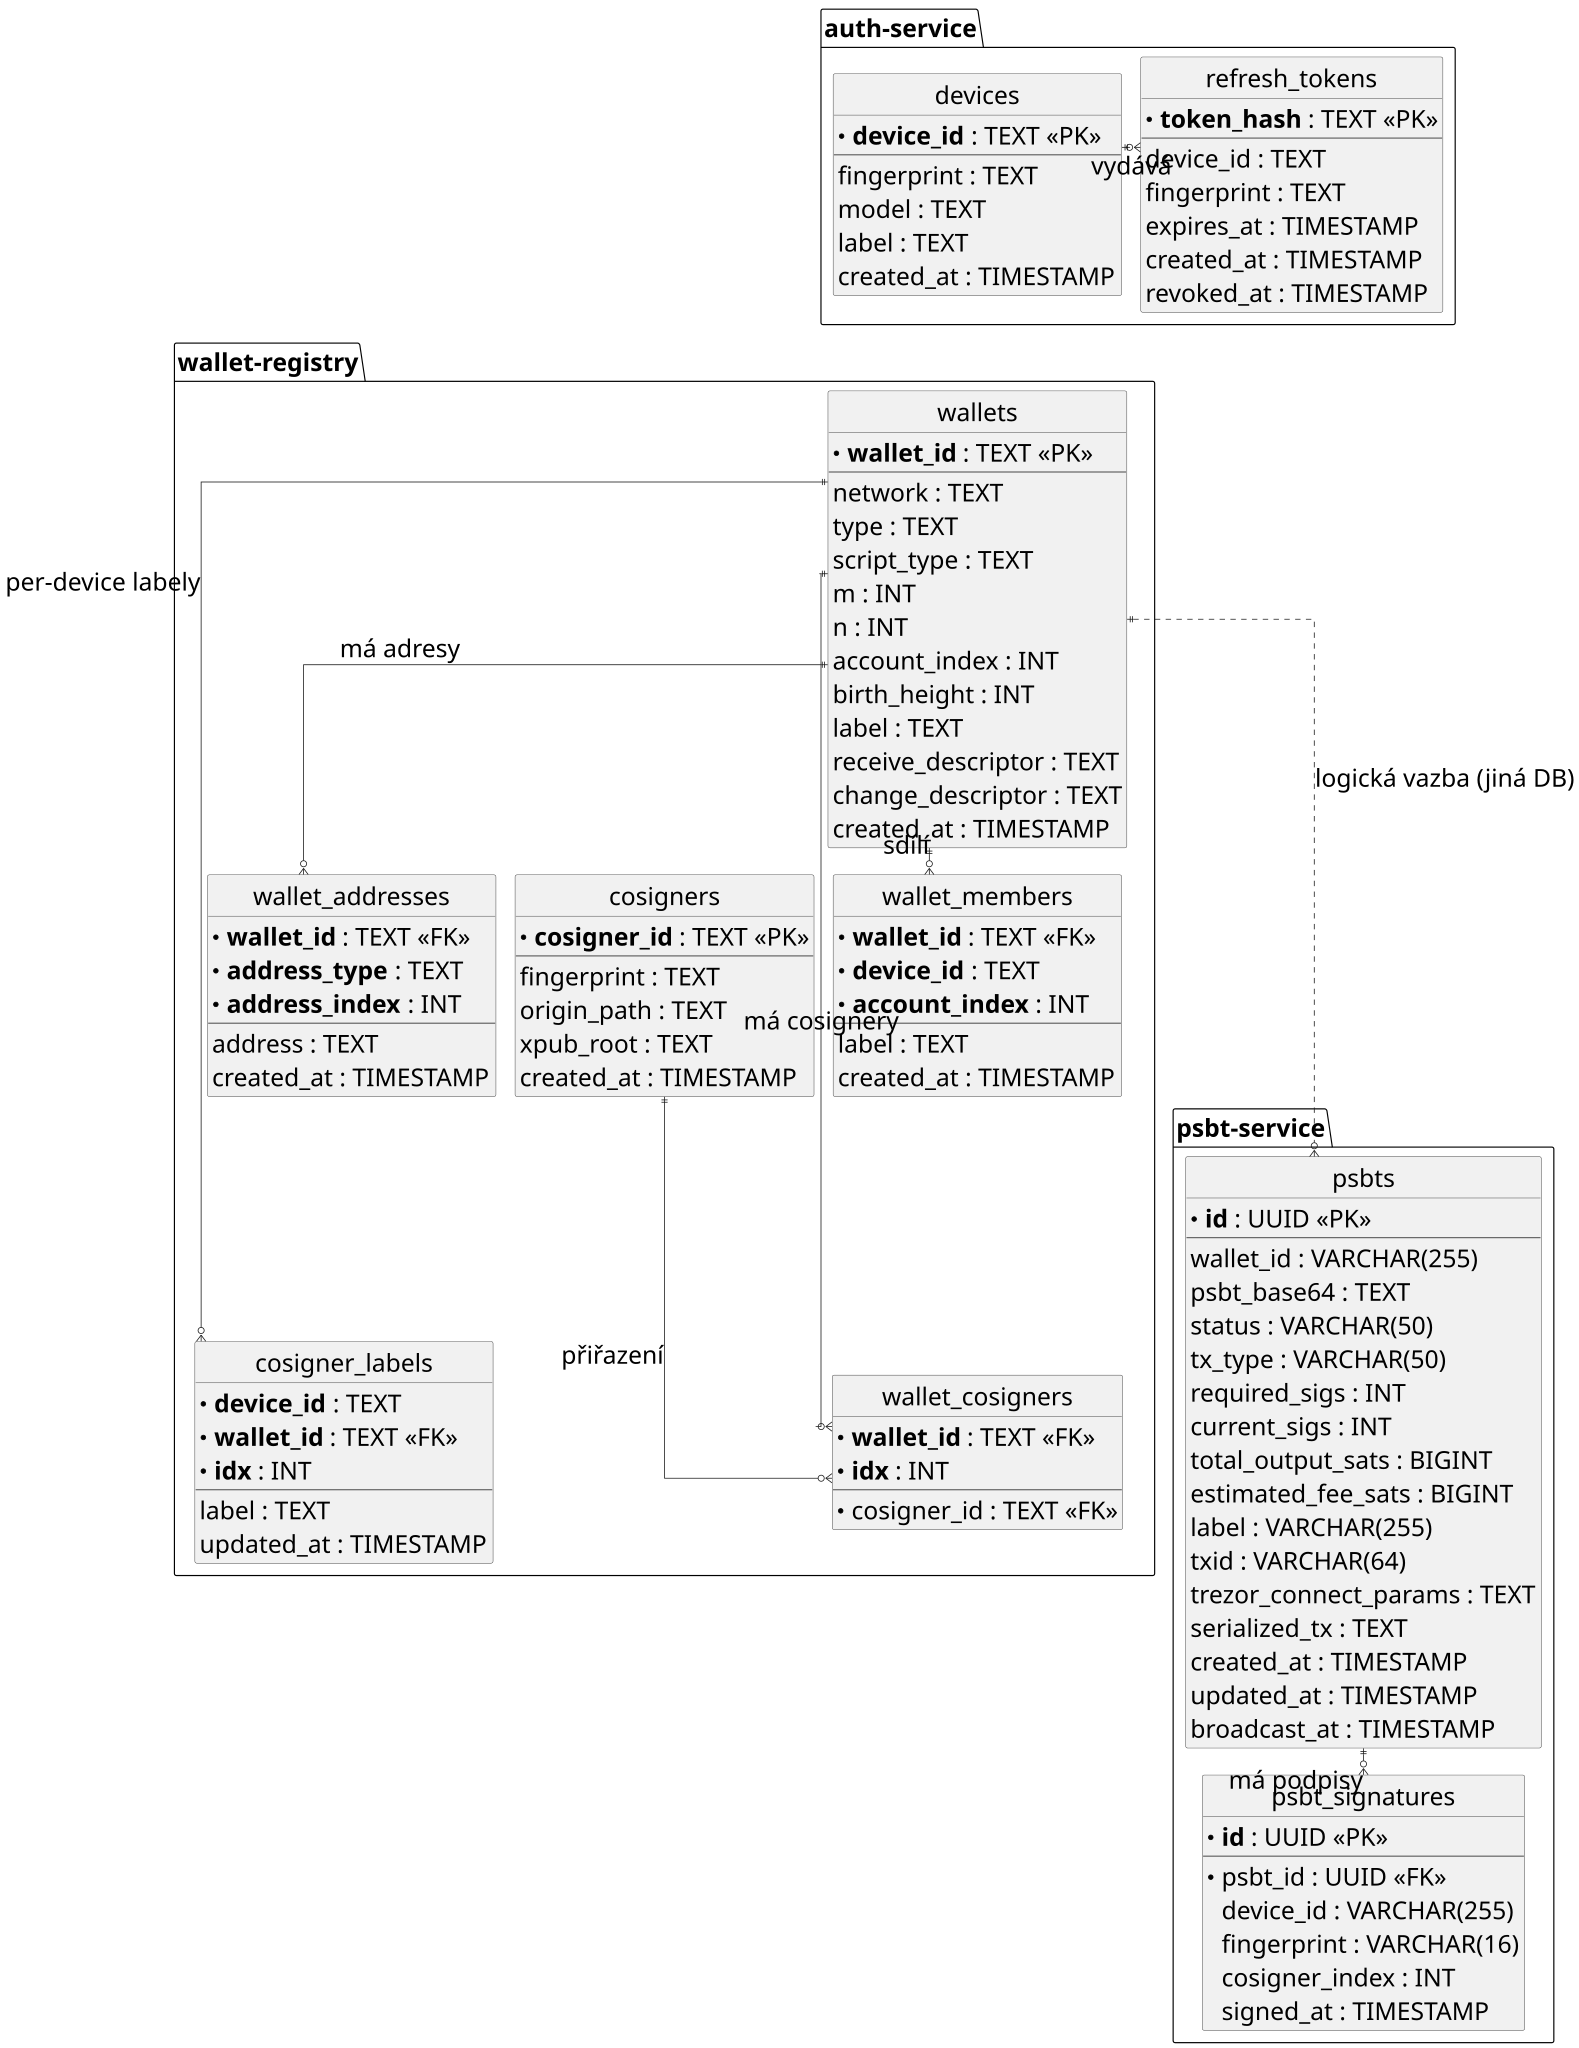
\includegraphics[width=\textwidth]{img/er-diagram.pdf}
\caption{ER diagram datového modelu. Databáze auth-service obsahuje tabulky
zařízení a~refresh tokenů, wallet-registry spravuje peněženky, cosignery,
adresy a~per-device labely, psbt-service uchovává PSBT transakce a~záznamy
podpisů.}
\label{fig:er-diagram}
\end{figure}

\subsection{Databáze PSBT služby}

Databáze \texttt{psbt-service} uchovává transakce v~různých fázích
jejich životního cyklu:

\begin{description}
\item[\texttt{psbts}] -- Hlavní tabulka PSBT transakcí. Obsahuje
  \texttt{id} (UUID, primární klíč),
  \texttt{wallet\_\allowbreak id} (odkaz na~peněženku),
  \texttt{psbt\_\allowbreak base64} (serializovaná PSBT ve~formátu
  Base64), \texttt{status} (pending~/~signed~/~broadcast),
  \texttt{required\_\allowbreak sigs} (požadovaný počet podpisů,
  tj.~$M$), \texttt{current\_\allowbreak sigs} (aktuální počet
  sebraných podpisů),
  \texttt{trezor\_\allowbreak connect\_\allowbreak params} (JSON
  s~parametry pro Trezor Connect, serializovaný do~sloupce typu TEXT)
  a~\texttt{serialized\_\allowbreak tx} (kompletní serializovaná
  transakce po~podpisu, pokud je dostupná).

\item[\texttt{psbt\_\allowbreak signatures}] {\sloppy -- Sleduje, kteří
  cosigneři již PSBT podepsali. Obsahuje
  \texttt{psbt\_\allowbreak id} (cizí klíč na \texttt{psbts.id}),
  \texttt{device\_\allowbreak id} (zařízení, které podepsalo),
  \texttt{fingerprint} (otisk kořenového klíče)
  a~\texttt{cosigner\_\allowbreak index} (index cosignera v~rámci
  peněženky). Tato tabulka zabraňuje duplicitnímu podpisu stejným
  cosignerem.\par}
\end{description}

Parametry pro Trezor Connect ukládáme jako serializovaný JSON
v~textovém sloupci. Jejich struktura závisí na~konkrétní transakci --
počet vstupů a~výstupů se liší, každý vstup má jinou derivační cestu
a~částku~--, ale přes SQL je nikdy nedotazujeme; celý dokument čte
pouze klient, a~to vždy vcelku. Strukturované dotazy a~indexace
(PostgreSQL typ \texttt{JSONB}) by zde proto nepřinesly žádnou výhodu,
a~relační reprezentace by zase vyžadovala zbytečně složité schéma
s~více vazebnými tabulkami. Prostý TEXT je v~tomto případě nejvhodnější
kompromis.

S~tabulkou \texttt{psbts} souvisí ještě jedna nezřejmá implementační
otázka. Při sestavování PSBT si \texttt{psbt-service} eviduje, která UTXO
peněženky jsou aktuálně rezervovaná v~rozpracovaných transakcích, a~při
volbě vstupů pro novou PSBT je vylučuje z~výběru. Bez této rezervace by
mohly vzniknout dvě konkurenční PSBT utrácející tytéž UTXO, z~nichž by
síť přijala jen jednu a~druhá by uvízla v~UI jako zdánlivě platná, ale
trvale nebroadcastovatelná transakce. Rezervace má ale nepříjemný
vedlejší efekt: pokud cosigner u~multisig peněženky nikdy nedokončí
podpis, opuštěný draft drží své vstupy zablokované navždy. Pro řešení
běží v~rámci \texttt{psbt-service} periodická úklidová úloha
(coroutine), která jednou za hodinu odstraní záznamy ve~stavech
\texttt{pending} a~\texttt{signed} starší než sedm dní; broadcastované
transakce zůstávají v~tabulce zachovány jako auditní stopa. Hodnoty
TTL i~intervalu jsou konfigurovatelné přes proměnné prostředí
(\texttt{PSBT\_TTL\_DAYS}, \texttt{PSBT\_CLEANUP\_INTERVAL\_MINUTES}),
celý mechanismus lze pro účely testování vypnout proměnnou
\texttt{PSBT\_CLEANUP\_ENABLED=false}. Uživatel může rozpracovaný draft
také kdykoliv ručně zrušit z~detailu PSBT v~mobilní aplikaci, což má
stejný efekt jako úklidová úloha (smazání řádku, uvolnění
rezervace).

%% -----------------------------------------------------------------------
\section{Návrh PSBT workflow}
\label{sec:psbt-workflow}

Formát PSBT a~zdůvodnění jeho volby pro koordinaci podepisování jsme
popsali v~sekcích~\ref{sec:psbt} a~\ref{sec:analyza-psbt}. Tato sekce
popisuje konkrétní návrh workflow -- jakým způsobem PSBT prochází
systémem od vytvoření po broadcast, jaké stavy nabývá a~jak se liší
singlesig a~multisig flow.

\subsection{Singlesig workflow}

V~případě singlesig peněženky (typ P2WPKH, BIP-84~\cite{BIP84}) probíhá
workflow transakcí ve třech krocích:

\begin{enumerate}
\item \textbf{Vytvoření PSBT} -- Uživatel zadá cílovou adresu, částku
  a~úroveň poplatku. \texttt{psbt-service} vybere UTXO (automaticky nebo
  manuálně dle volby uživatele), sestaví transakci, vypočítá poplatek
  a~vytvoří PSBT včetně parametrů pro Trezor Connect.
\item \textbf{Podpis na Trezoru} -- Mobilní aplikace otevře Trezor Suite
  Mobile s~parametry transakce. Uživatel potvrdí podpis na hardwarové
  peněžence. Trezor vrátí kompletní serializovanou transakci.
\item \textbf{Broadcast} -- Aplikace odešle serializovanou transakci
  na backend, který ji přes \texttt{blockchain-service} propaguje
  do Bitcoinové sítě.
\end{enumerate}

\subsection{Multisig workflow}

Multisig peněženka (typ P2WSH, BIP-48~\cite{BIP48}) ve schématu $M$-of-$N$
vyžaduje podpisy od $M$ z~$N$ cosignerů. Workflow se liší od singlesig
v~tom, že po podpisu prvním cosignerem transakce ještě není kompletní:

\begin{enumerate}
\item \textbf{Vytvoření PSBT} -- Stejné jako u~singlesig. PSBT je uloženo
  se statusem \texttt{pending} a~s~\texttt{current\_sigs = 0}.
\item \textbf{Podpis cosignerem $i$} -- Cosigner otevře detail PSBT v~aplikaci,
  přepne na svůj účet (odpovídající jeho derivační cestě) a~podepíše na
  svém Trezoru. Trezor Connect vrací jak pole podpisů, tak
  \texttt{serializedTx}. Backend z~odpovědi extrahuje pole podpisů,
  uloží je a~inkrementuje \texttt{current\_sigs}.
\item \textbf{Opakování} -- Kroky se opakují pro další cosignery, dokud
  není dosažen práh \texttt{current\_sigs == required\_sigs} ($M$).
\item \textbf{Broadcast} -- Po dosažení prahu je PSBT připraveno k~odeslání.
  Uživatel z~detailu PSBT zvolí broadcast a~backend transakci finalizuje
  a~propaguje do Bitcoin sítě.
\end{enumerate}

Celý multisig podepisovací flow zachycují sekvenční diagramy na
obrázcích~\ref{fig:multisig-signing-1} a~\ref{fig:multisig-signing-2}.

\begin{figure}[htbp]
\centering
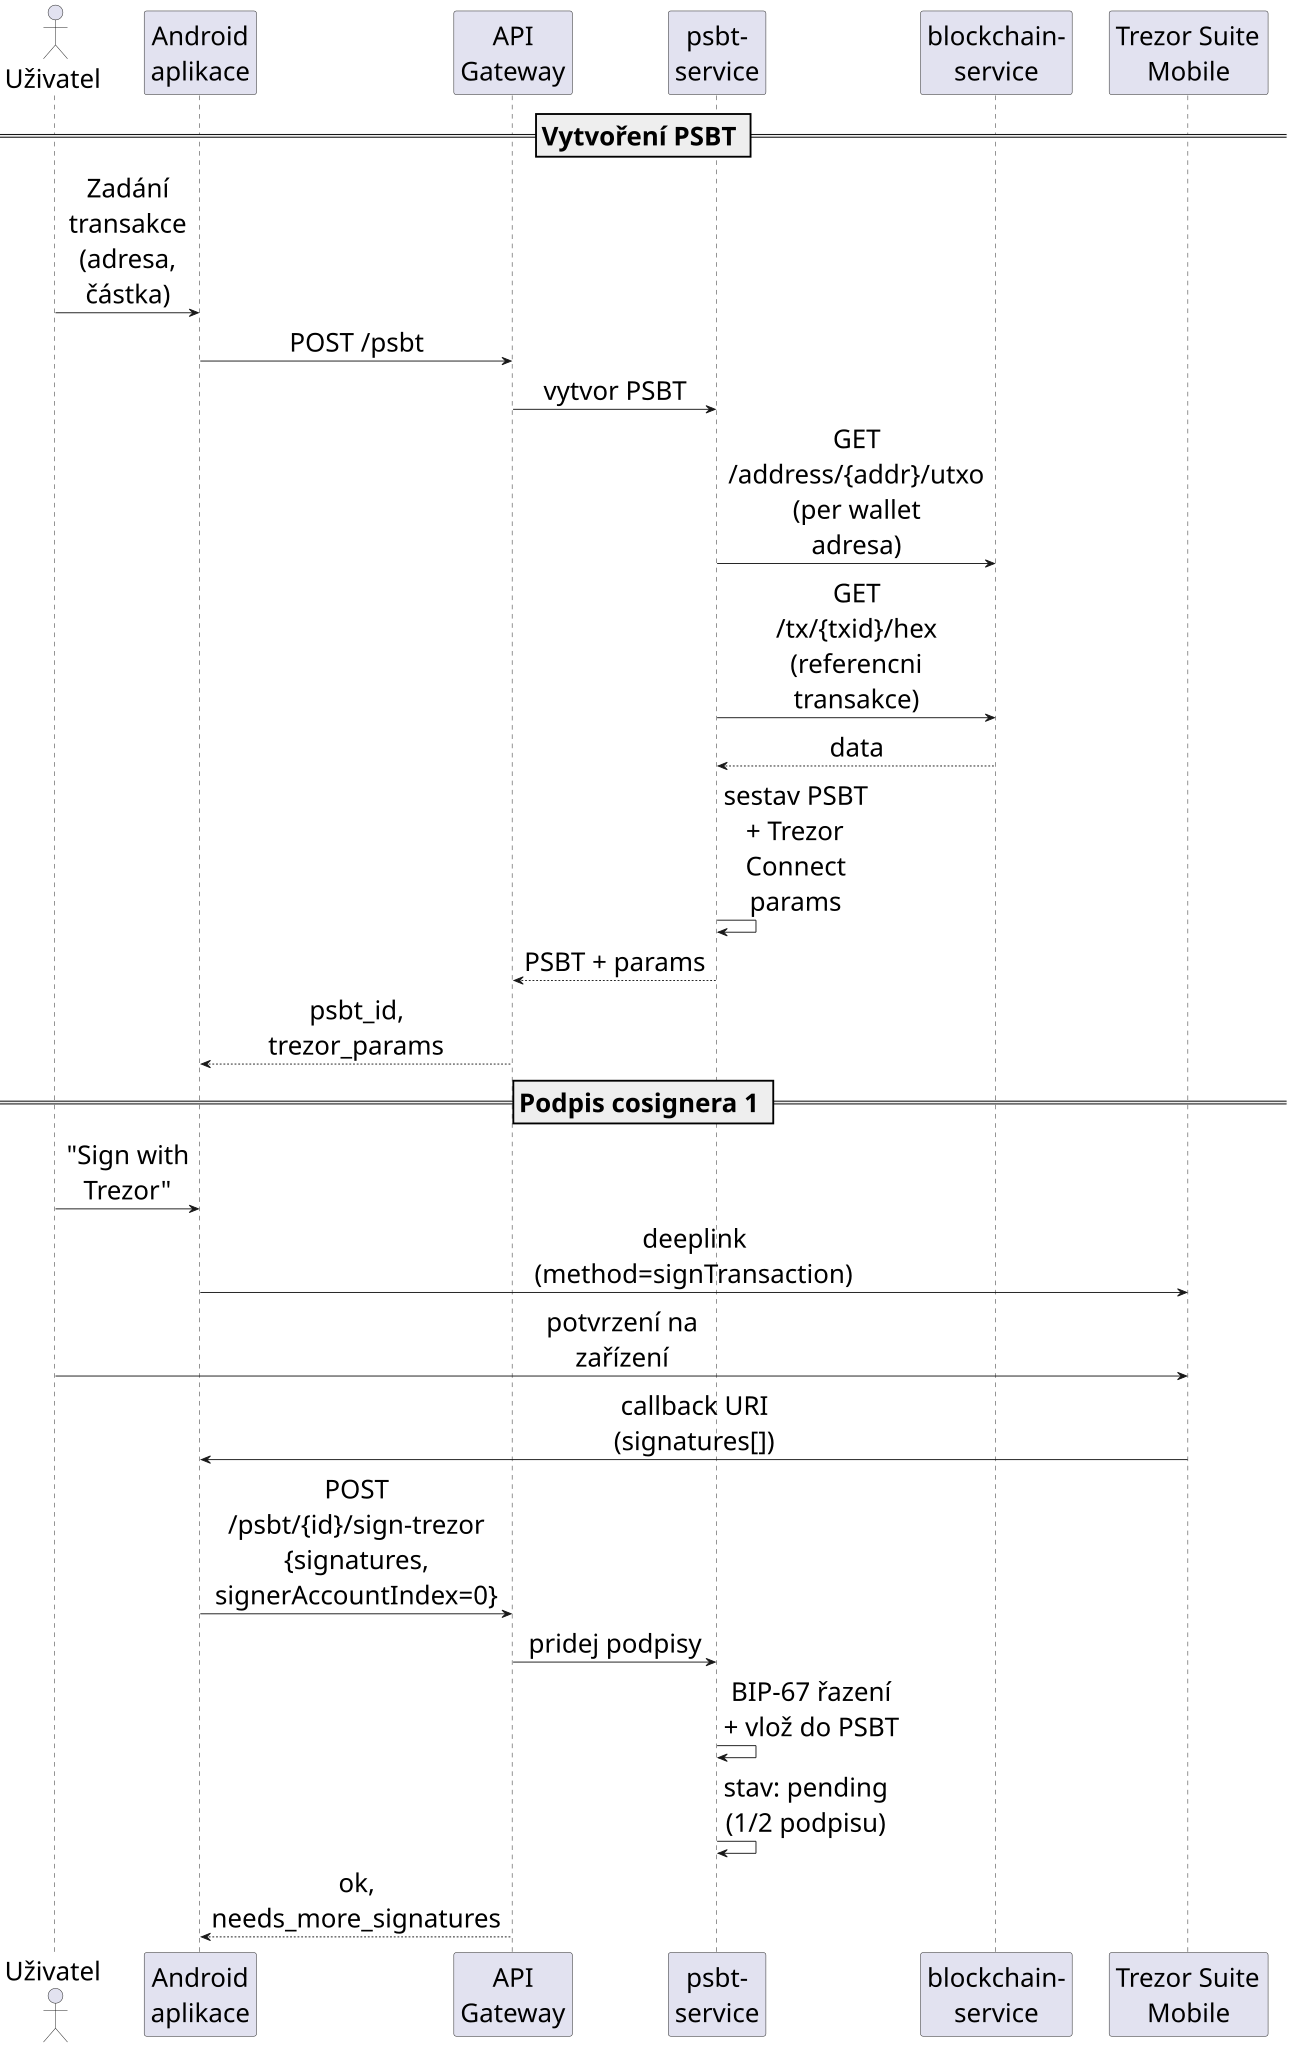
\includegraphics[width=\textwidth,height=0.85\textheight,keepaspectratio]{img/multisig-signing-1.pdf}
\caption{Sekvenční diagram 2-of-3 multisig podepisování -- první část:
vytvoření PSBT a~podpis prvním cosignerem. Backend sestaví PSBT,
mobilní aplikace deleguje podpis na Trezor Suite Mobile a~přidá první podpis.}
\label{fig:multisig-signing-1}
\end{figure}

\begin{figure}[htbp]
\centering
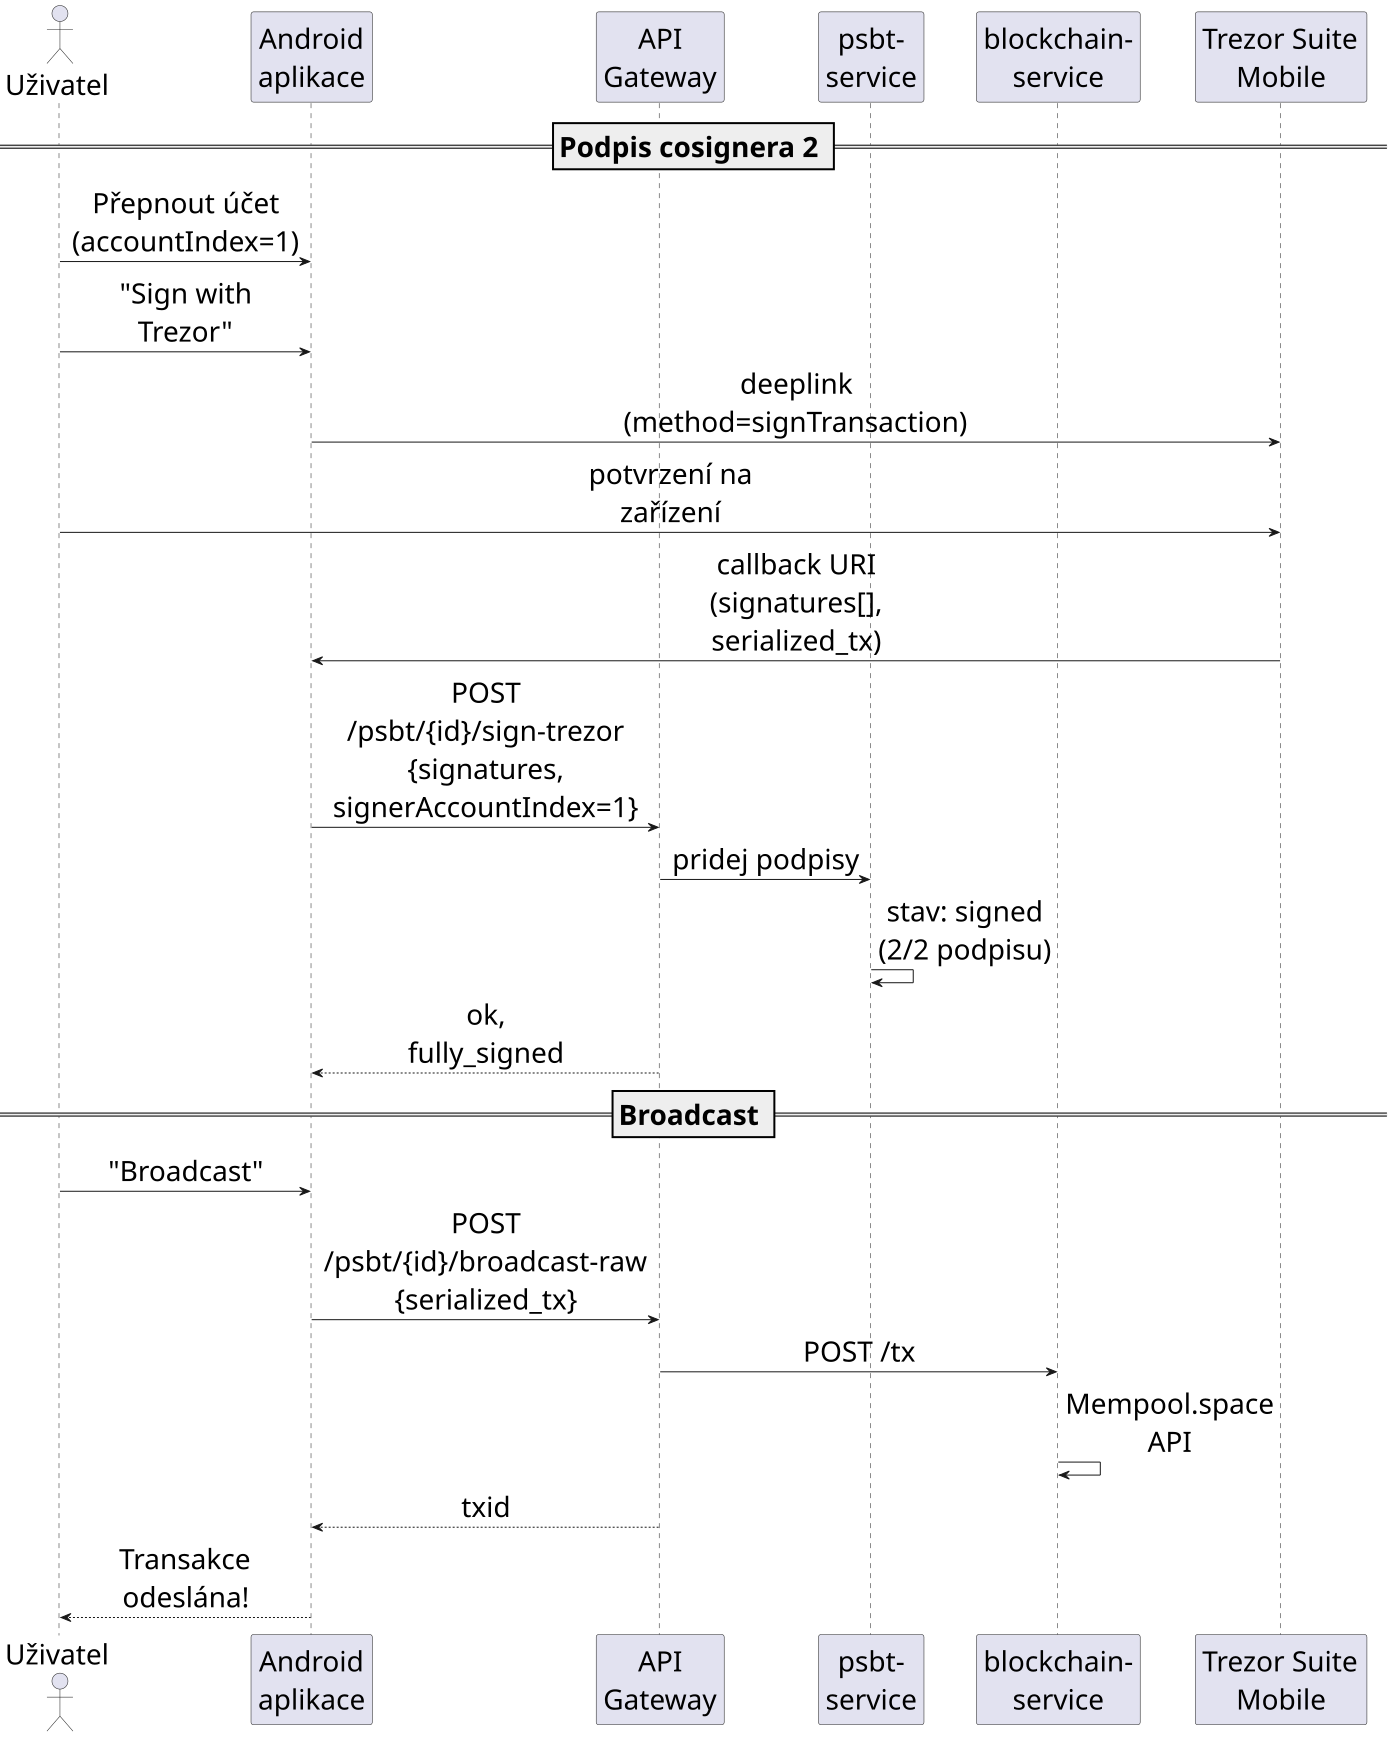
\includegraphics[width=\textwidth,height=0.85\textheight,keepaspectratio]{img/multisig-signing-2.pdf}
\caption{Sekvenční diagram 2-of-3 multisig podepisování -- druhá část:
podpis druhým cosignerem a~broadcast finální transakce. Po dosažení
prahu podpisů uživatel zvolí broadcast a~backend transakci finalizuje
a~odešle do Bitcoinové sítě.}
\label{fig:multisig-signing-2}
\end{figure}

Alternativní přístup k~multisig podepisování by bylo předávání PSBT
souboru mezi cosignery (například prostřednictvím QR kódů nebo SD karet),
jak to implementuje například Sparrow Wallet~\cite{SparrowWallet}. Tento
\emph{offline} přístup je bezpečnější z~hlediska soukromí, protože nevyžaduje
centrální server. V~kontextu mobilní aplikace je však nepraktický --
uživatel by musel manuálně exportovat a~importovat PSBT soubory. Zvolený
serverový přístup umožňuje, aby cosigneři jednoduše otevřeli seznam
čekajících transakcí v~aplikaci a~podepsali jedním kliknutím.

\subsection{Výběr UTXO a coin control}
\label{subsec:coin-control}

Při tvorbě transakce je nutné vybrat, které nepoužité výstupy (UTXO) budou
použity jako vstupy. Aplikace nabízí dva režimy:

\begin{description}
\item[Automatický výběr] -- Systém vybírá UTXO strategií \emph{largest-first}:
  řadí dostupné UTXO sestupně podle hodnoty a~přidává je, dokud součet
  nepřekročí požadovanou částku včetně poplatku. Tato strategie minimalizuje
  počet vstupů (a~tedy velikost a~poplatek transakce), ale může vést
  k~suboptimálnímu výběru z~hlediska soukromí, protože spojuje velké UTXO.

\item[Manuální výběr (coin control)] -- Uživatel sám vybírá konkrétní UTXO,
  které chce utratit. Tato pokročilá funkce umožňuje uživateli řídit, které
  adresy a~částky vstupují do transakce, což je důležité pro zachování
  soukromí (zamezení spojování UTXO z~různých zdrojů) a~pro řízení
  konsolidace prostředků.
\end{description}

Zvažovali jsme i~pokročilejší algoritmy výběru UTXO, jako je
\emph{Branch and Bound} (používaný v~Bitcoin Core), který hledá přesný součet
bez nutnosti change výstupu. Pro první verzi aplikace jsme zvolili jednodušší
strategii \emph{largest-first}, která je dostatečná pro většinu případů
použití a~je snadno předvídatelná pro uživatele.

\subsection{Výpočet poplatku}

Poplatek za transakci se v~Bitcoin síti odvíjí od velikosti transakce
ve virtuálních bytech (vBytes), nikoliv od převáděné částky. Virtuální
velikost se dle BIP-141~\cite{BIP141} vypočítá jako:

\[
\mathit{vSize} = \left\lceil \frac{\mathit{weight}}{4} \right\rceil, \quad
\mathit{weight} = \mathit{base\_size} \times 3 + \mathit{total\_size}
\]

\noindent kde \emph{base\_size} je velikost transakce bez witness dat
a~\emph{total\_size} zahrnuje i~witness. Díky tomuto vzorci mají witness
data (podpisy) čtyřikrát nižší váhu než ostatní části transakce, což je
motivace pro přechod na SegWit adresy.

Odhad velikosti závisí na typu peněženky:

\begin{itemize}
\item \textbf{P2WPKH (singlesig)} -- každý vstup přidá přibližně 68~vB
  (41~B non-witness: outpoint 36~B, sequence 4~B, délka skriptu 1~B;
  plus witness: 1~B počet položek, ${\approx}72$~B DER podpis,
  33~B komprimovaný veřejný klíč). Každý výstup přidá přibližně 31~vB
  a~fixní režie transakce (verze, počty, locktime) činí přibližně 10~vB.

\item \textbf{P2WSH (multisig)} -- vstup je výrazně větší, protože
  witness musí obsahovat $M$~podpisů a~kompletní redeem skript s~$N$
  veřejnými klíči. Non-witness část zůstává 41~B, ale witness data
  rostou: úvodní \texttt{OP\_0} (${\approx}6$~B s~délkami), $M$~podpisů
  (každý maximálně 73~B: DER-kódovaný ECDSA podpis plus push opcode)
  a~redeem skript ($N \times 34$~B pro komprimované veřejné klíče plus
  opcodes \texttt{OP\_M}, \texttt{OP\_N}, \texttt{OP\_CHECKMULTISIG}).
  Velikost vstupu odhadujeme dle výpočtu popsaného
  v~sekci~\ref{sec:p2wsh-multisig} jako $41 + (6 + 73M + 34N)/4$~vB.
  Například pro schéma 2-of-3: $41 + (6 + 146 + 102)/4 \approx 105$~vB
  na vstup.
\end{itemize}

Celková odhadovaná velikost transakce je tedy:

\[
\mathit{vSize}_{\text{odhad}} = \text{režie} + n_{\text{vstupů}} \times \mathit{vSize}_{\text{vstup}} + n_{\text{výstupů}} \times 31 \;\text{vB}
\]

\noindent Tato hodnota se vynásobí aktuální sazbou poplatku (v~sat/vB),
kterou uživatel volí z~nabídky tří úrovní: nízký poplatek (odhad pro
potvrzení do jedné hodiny), střední (do třiceti minut) a~vysoký (nejbližší
blok). Sazby pro jednotlivé úrovně aplikace získává z~blockchainového API,
které je odvozuje z~aktuálního stavu mempoolu -- fronty nepotvrzených
transakcí čekajících na zařazení do bloku~\cite{MempoolAPI}. V~režimu
manuálního výběru UTXO může uživatel alternativně zadat libovolnou sazbu
v~sat/vB ručně.

\subsection{Zpracování change výstupu}

Pokud součet vybraných UTXO překračuje požadovanou částku včetně poplatku,
vytvoří se change výstup vracející přebytek zpět do peněženky na novou
change adresu. Existuje však speciální případ: pokud by hodnota change
výstupu byla menší než tzv.~\emph{dust threshold}, change výstup se
nevytváří a~celý přebytek se přidá k~poplatku. Vytvořením výstupu pod
prahem by transakce nebyla standardní a~uzly v~síti by ji odmítly propagovat.
Dust threshold závisí na typu výstupu: pro P2PKH je 546~satoshi,
pro P2WPKH 294~satoshi a~pro P2WSH 330~satoshi. V~implementaci
používáme konzervativní hodnotu 546~satoshi bez ohledu na typ výstupu,
čímž garantujeme, že žádný výstup nebude uzly odmítnut.

%% -----------------------------------------------------------------------
\section{Návrh uživatelského rozhraní}
\label{sec:ui-navrh}

\subsection{Architektonický vzor MVVM}

Pro organizaci kódu mobilní aplikace jsme zvolili architektonický vzor
MVVM (\emph{Model--View--ViewModel}), který je doporučeným přístupem
pro Android aplikace s~Jetpack Compose. Jednotlivé vrstvy mají tyto role:

\begin{description}
\item[Model] -- Datové třídy reprezentující doménové entity (peněženka,
  transakce, UTXO, PSBT) a~repozitáře zajišťující komunikaci s~backendem
  prostřednictvím REST API.
\item[ViewModel] -- Obsahuje prezentační logiku a~udržuje stav obrazovky.
  Stav je reprezentován Kotlinovým \texttt{StateFlow}, na jehož změny
  se Compose UI automaticky přehlásí a~překreslí dotčené komponenty.
  ViewModel přežívá změnu konfigurace (otočení obrazovky) díky integraci
  s~Android lifecycle.
\item[View (Composable)] -- Deklarativní Compose funkce, které vykreslují
  UI na základě stavu z~ViewModelu. Neobsahují žádnou business logiku
  a~jsou snadno testovatelné a~znovupoužitelné.
\end{description}

Alternativou by byl vzor MVI (\emph{Model--View--Intent}), který je
přísnější v~tom, že veškeré uživatelské akce modeluje jako unidirektionální
proud intentů. MVI nabízí lepší predikovatelnost stavu, ale za cenu vyššího
množství boilerplate kódu. Pro rozsah aplikace je MVVM dostatečný
a~lépe odpovídá konvencím Android ekosystému.

\subsection{Navigační struktura}

Navigace v~aplikaci sleduje lineární tok s~možností návratu:

\begin{enumerate}
\item \textbf{Připojení Trezoru} -- Úvodní obrazovka, kde uživatel připojí
  Trezor přes deeplink do Trezor Suite Mobile. Aplikace vyžádá export xpub
  pro deset účtů (BIP-84).
\item \textbf{Skenování účtů} -- Backend provede account discovery, ověří
  aktivitu na blockchainu a~vytvoří singlesig peněženky pro účty
  s~transakční historií.
\item \textbf{Výběr singlesig účtu} -- Uživatel vybere jeden ze singlesig
  účtů odvozených z~Trezoru. Multisig peněženky se zde nezobrazují --
  ty jsou přidružené k~singlesig účtům a~přístupné přes navigační menu.
\item \textbf{Dashboard} -- Hlavní obrazovka zobrazující zůstatek vybraného
  singlesig účtu (v~BTC i~ve zvolené fiat měně), seznam transakcí
  a~tlačítka pro odeslání a~příjem. Postranní navigační menu
  (\emph{drawer}) umožňuje přechod na seznam multisig peněženek
  a~nastavení.
\item \textbf{Multisig peněženky} -- Seznam importovaných multisig peněženek
  přidružených k~aktuálnímu zařízení. Po výběru peněženky se zobrazí
  její vlastní dashboard se zůstatkem, transakcemi a~přístupem
  k~seznamu PSBT transakcí.
\end{enumerate}

Přehled navigační struktury a~přechodů mezi obrazovkami zachycuje
obrázek~\ref{fig:navigation}.

\begin{figure}[htbp]
\centering
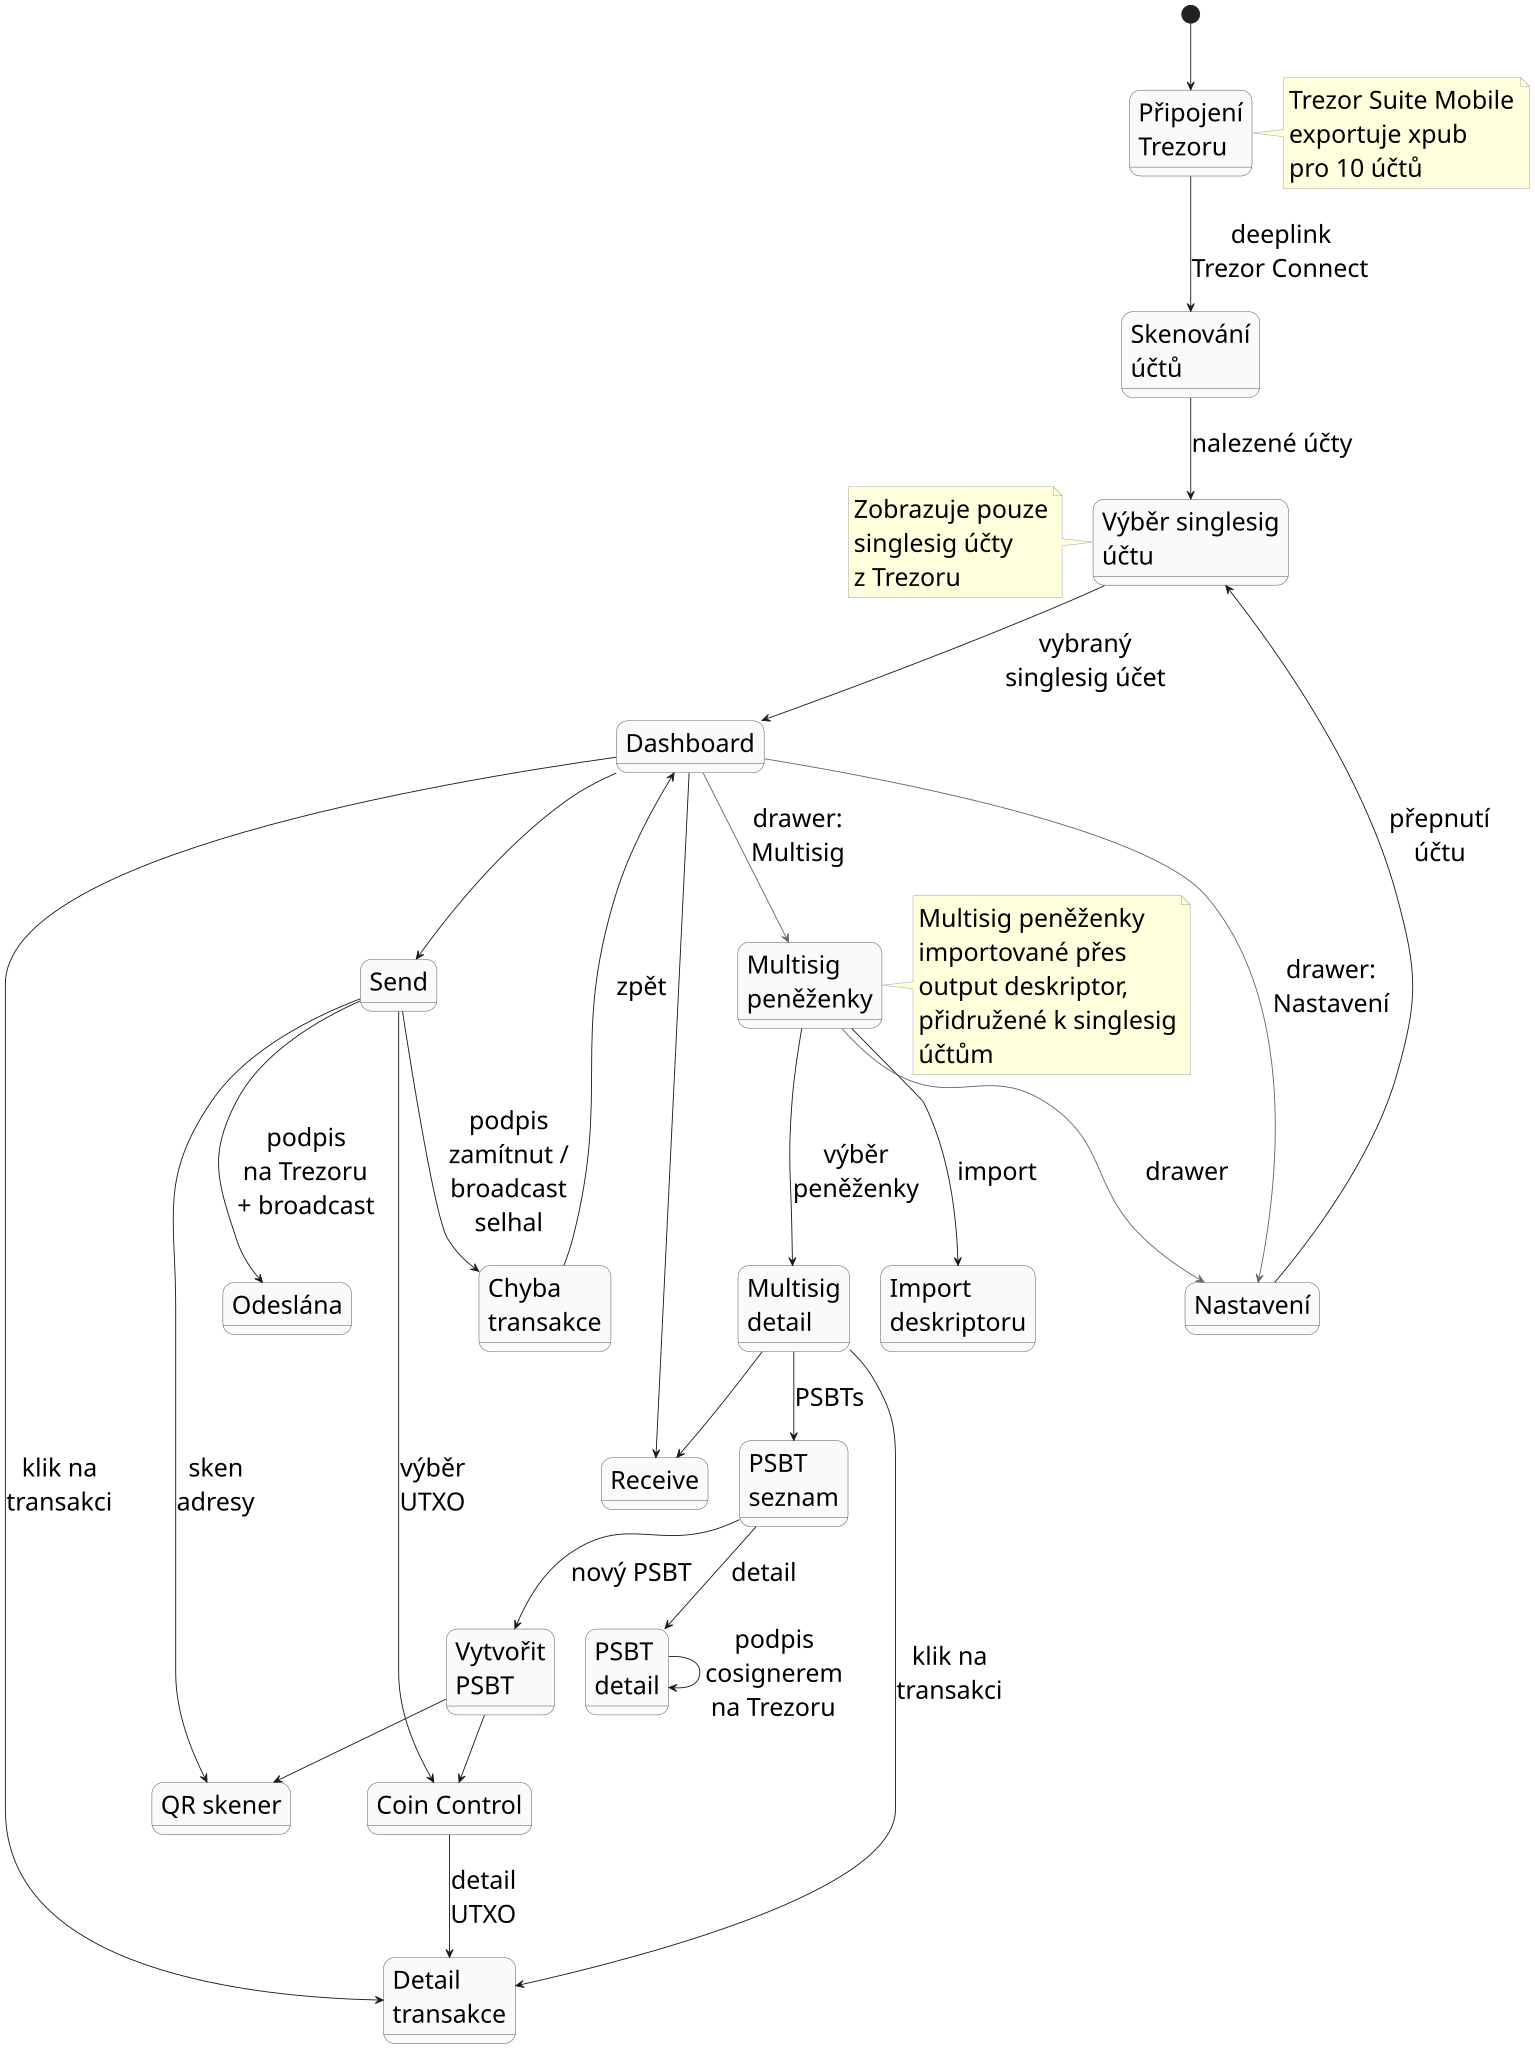
\includegraphics[width=\textwidth]{img/navigation.pdf}
\caption{Navigační diagram aplikace. Po připojení Trezoru uživatel vybere
singlesig účet a~vstoupí na dashboard. Multisig peněženky jsou přístupné
přes postranní menu a~mají vlastní detail se seznamem PSBT. Šedé šipky
značí navigaci přes drawer menu.}
\label{fig:navigation}
\end{figure}

\subsection{Klíčové obrazovky}

\begin{description}
\item[Dashboard] -- Zobrazuje zůstatek peněženky, konverzi do fiat měny
  a~chronologický seznam transakcí s~potvrzeními. Pro multisig peněženku
  navíc zobrazuje počet čekajících PSBT vyžadujících podpis.

\item[Detail transakce] -- Rozklikem libovolné položky ze seznamu
  transakcí na dashboardu. Zobrazuje \texttt{txid}, stav potvrzení, výšku
  bloku, časové razítko, poplatek včetně sazby v~sat/vB a~seznam vstupů
  a~výstupů s~částkami. Adresy patřící aktuální peněžence jsou označeny
  štítkem \emph{YOURS}. Kliknutím na vstup lze otevřít předchozí transakci,
  která daný UTXO vytvořila, a~procházet tak historii až do hloubky pěti
  úrovní; na každé úrovni je štítkem \emph{FROM HERE} označen výstup, který
  navazuje na proklikaný vstup z~úrovně předchozí. Hloubka je omezená,
  aby nedošlo k~nadměrnému zatížení blockchainového API. Tato funkce slouží
  uživateli k~forenznímu ověření původu prostředků bez nutnosti přepínat
  do externího prohlížeče blockchainu.

\item[Send (odeslání)] -- Formulář pro zadání cílové adresy (manuálně
  nebo skenováním QR kódu), částky, volby úrovně poplatku a~volitelně
  manuálního výběru UTXO (coin control). Po vyplnění formuláře se zobrazí
  souhrn transakce a~uživatel potvrdí odeslání, čímž se zahájí podepisování
  na Trezoru.

\item[Receive (příjem)] -- Zobrazuje aktuální přijímací adresu peněženky
  ve formě QR kódu a~textového řetězce s~možností kopírování do schránky.
  Tlačítko \emph{Zobrazit na Trezoru} umožňuje ověřit adresu na displeji
  hardwarové peněženky (viz popis v~sekci~\ref{subsec:trezor-connect}).

\item[PSBT seznam] -- Přístupný pouze pro multisig peněženky. Zobrazuje
  seznam vytvořených PSBT transakcí s~jejich stavem (čekající na podpisy /
  podepsaná / broadcastovaná). U~čekajících transakcí zobrazuje, kolik
  podpisů zbývá do prahu.

\item[PSBT detail] -- Detail konkrétní PSBT transakce se souhrnem částky,
  poplatku a~celkové hodnoty. Zobrazuje stav podpisů jednotlivých cosignerů --
  u~každého cosignera je vidět, zda podepsal, a~v~dialogu signerů si uživatel
  může cosignerům přiřadit vlastní pojmenování (například ,,Alicin klíč``).
  Tento název je privátní pro dané zařízení -- uloží se vázaný na
  \texttt{device\_id} přihlášeného Trezoru a~ostatním cosignerům se nezobrazí.
  Důvodem je ochrana soukromí: osobní poznámky o~spolupodepisovatelích by
  neměly prosakovat mezi členy sdílené peněženky. Pokud transakce čeká
  na podpis aktuálního cosignera, zobrazí se tlačítko pro podepsání.

\item[Nastavení] -- Umožňuje přepnutí aktivního účtu (pro multisig testování
  s~více cosignery na jednom zařízení), výběr fiat měny pro zobrazení
  ekvivalentu zůstatku (CZK, USD nebo EUR), import output deskriptoru pro
  vytvoření multisig peněženky a~zobrazení informací o~aplikaci
  a~připojeném zařízení.
\end{description}

Při návrhu obrazovek jsme kladli důraz na přehlednost a~bezpečnost.
Před odesláním každé transakce se zobrazí kompletní souhrn (cílová adresa,
částka, poplatek), aby uživatel měl poslední možnost ověřit správnost
údajů před potvrzením na hardwarové peněžence. Detaily transakce
uživatel vždy ověřuje ještě na displeji samotného Trezoru, což poskytuje
nezávislou kontrolu proti případné kompromitaci mobilní aplikace.

%% -----------------------------------------------------------------------
\section{Implementační detaily}
\label{sec:impl-detaily}

V~této sekci popisujeme vybrané implementační problémy a~technické výzvy,
které přesahují rámec architektonického návrhu a~které považujeme
za zajímavé z~hlediska pochopení fungování systému.

\subsection{Sestavení binární struktury PSBT}

Třída \texttt{PsbtBuilder} v~modulu \texttt{psbt-service} sestavuje kompletní
binární strukturu PSBT dle BIP-174~\cite{BIP174}. Formát začíná magic sekvencí
\texttt{0x70736274ff} (ASCII \uv{psbt} + separátor), následovanou globální sekcí
s~nepodepsanou transakcí, per-input sekcemi s~metadaty pro podepisování
a~per-output sekcemi s~derivačními cestami. Každá sekce je ukončena nulovým bajtem.

Pro každý vstup zapisujeme čtyři typy záznamů:
\begin{itemize}
\item \texttt{PSBT\_IN\_NON\_WITNESS\_UTXO} -- celá předchozí transakce v~raw
  formátu. Firmware Trezor od verze~2.3.1 vyžaduje tento záznam i~pro nativní
  SegWit vstupy~\cite{TrezorFirmwareDocs}, aby mohl ověřit částky vstupů
  a~zobrazit správný poplatek.
\item \texttt{PSBT\_IN\_WITNESS\_UTXO} -- částka a~scriptPubKey utrácené UTXO.
\item \texttt{PSBT\_IN\_WITNESS\_SCRIPT} -- witness skript multisig transakce
  (pouze pro P2WSH) se~všemi veřejnými klíči v~BIP-67 pořadí.
\item \texttt{PSBT\_IN\_BIP32\_DERIVATION} -- derivační cesta pro každého
  cosignera, aby Trezor identifikoval svůj klíč.
\end{itemize}

\noindent Pro change výstup přidáváme \texttt{PSBT\_OUT\_BIP32\_DERIVATION},
aby peněženka rozpoznala, že change směřuje zpět na~vlastní adresu.

\subsection{Převod PSBT na parametry Trezor Connect}

Trezor Connect nepřijímá PSBT přímo -- vyžaduje strukturovaný JSON
s~explicitními derivačními cestami, multisig metadaty a~referenčními
transakcemi~\cite{TrezorConnect,TrezorFirmwareDocs}. Třída
\texttt{TrezorParamsBuilder} provádí tento převod.

Pro singlesig transakce je převod přímočarý: každý vstup obsahuje
derivační cestu jako pole uint32 hodnot (hardened indexy s~bitem
\texttt{0x80000000}), hash a~index předchozí transakce, částku a~typ
skriptu. Change výstup místo cílové adresy obsahuje derivační cestu,
aby Trezor poznal interní výstup.

Pro multisig transakce vyžaduje každý vstup navíc objekt \texttt{multisig}
obsahující pole \texttt{pubkeys} (strukturovaný \texttt{HDNodeType} místo
xpub řetězce), práh~$M$ a~pole \texttt{signatures} (prázdné řetězce pro
dosud nepodepsané pozice). Pořadí klíčů musí přesně odpovídat BIP-67
řazení pro daný vstup -- Trezor firmware řazení neprovádí interně.

Trezor Connect dále vyžaduje referenční transakce v~parsované podobě
(ne raw hex), proto backend pro každý vstup stáhne předchozí
transakci z~\texttt{blockchain-\allowbreak service} a~převede ji
na~strukturovaný formát s~poli \texttt{version}, \texttt{inputs},
\texttt{bin\_\allowbreak outputs} a~\texttt{lock\_\allowbreak time}.

\subsection{BIP-67 řazení podpisů ve witness}

Jednou z~nejobtížnějších chyb, na které jsme při vývoji narazili, bylo
správné řazení podpisů ve~witness stacku multisig transakce. Podpisy
musí být umístěny ve~stejném pořadí jako odpovídající veřejné klíče
ve~witness skriptu. Protože \texttt{sortedmulti} deskriptory řadí klíče
lexikograficky dle BIP-67~\cite{BIP67}, nemusí se~toto pořadí shodovat
s~pořadím cosignerů podle jejich indexu.

Původní implementace umísťovala podpis na~pozici odpovídající
\texttt{cosigner\-Index}. To fungovalo, pouze dokud se~lexikografické
pořadí náhodou shodovalo s~pořadím cosignerů. Chyba se~projevila
až při testování s~cosignerem, jehož veřejný klíč byl po~BIP-67 řazení
na~jiné pozici. Po~opravě systém pro každý vstup zvlášť odvodí child
pubkeys všech cosignerů, seřadí je lexikograficky a~podpis umístí
na~odpovídající pozici.

\subsection{Předcházení reuse change adres}

Další chyba, která se~projevila až při testování s~reálnými prostředky,
se~týkala výběru change adresy při sestavování PSBT. Původní implementace
volala \texttt{wallet-registry} s~pevně zadaným indexem~0, což znamenalo,
že \emph{každá} odchozí transakce posílala svůj change výstup na tutéž
adresu. Nebylo to okamžitě viditelné, protože adresa se~v~UI nikdy
nezobrazuje -- uživatel ji vidí jen v~prohlížeči blockchainu nebo při
detailním procházení historie. Při opakovaných odchozích transakcích
tak vznikal řetězec, kde se~stejná adresa opakovaně objevovala jako
vstup i~jako change výstup, což je anti-pattern z~hlediska soukromí:
pozorovatel blockchainu může všechny takové transakce triviálně spojit
do jediného klastru a~odhadnout celkový zůstatek i~aktivitu peněženky.

Oprava vyžadovala zavést novou komponentu pro výběr adres s~kontrolou
on-chain aktivity. Službu \texttt{explorer-service} jsme rozšířili
o~endpoint vracející první change adresu bez transakční historie, což
je analogie již existující logiky pro přijímací adresy. Pokud jsou
všechny adresy v~rámci počátečního gap limitu~20 již použité, zavolá
se~nově zavedený endpoint \texttt{wallet-registry} pro~odvození dalšího
indexu za gap limit a~jeho zápis do databáze. Služba \texttt{psbt-service}
si tak pro každou novou PSBT vyžádá čerstvou change adresu, a~řetězec
opakovaných výskytů byl definitivně rozbit.

\subsection{Rate limiting blockchainového API}

Služba \texttt{blockchain-service} řeší rate limiting
Mempool.space API, které při překročení souběžných požadavků vrací
HTTP~429. Při stahování dat pro celou peněženku (až 40~adres paralelně)
k~tomu snadno dojde. Implementovali jsme omezení pomocí Kotlin coroutine
\texttt{Semaphore} s~limitem 5~souběžných požadavků a~jedním retry
s~jednosekundovým zpožděním při selhání. Více pokusů záměrně neprovádíme --
pokud je IP adresa v~\uv{penalty box}, opakované pokusy pouze prodlužují
frontu.

\subsection{Agregace dat peněženky}

Služba \texttt{explorer-service} řeší tzv.\ N+1~problém: frontend potřebuje
zobrazit data celé peněženky (zůstatek, transakce, UTXO), ale blockchainové
API pracuje na~úrovni jednotlivých adres. Pro peněženku se 40~adresami
(20~receive + 20~change) by naivní přístup vyžadoval 40~HTTP volání.
Implementovali jsme dvoustupňovou optimalizaci: nejprve jedním lehkým
voláním zjistíme \texttt{tx\_count} pro každou adresu a~přeskočíme neaktivní,
poté pro aktivní adresy stahujeme detailní data paralelně. Tím se počet
volání typicky sníží na~5--10.

\subsection{Signing interface}

Jak jsme analyzovali v~sekci~\ref{sec:analyza-trezor}, architektura aplikace
je navržena s~čistým interním rozhraním pro podepisování. V~aktuální verzi
je implementováno prostřednictvím deeplinků do Trezor Suite Mobile, ale
abstrakce je připravena tak, aby bylo možné v~budoucnu přidat přímou USB
komunikaci s~Trezorem jako alternativní implementaci bez nutnosti změn
ve~zbytku systému. Třída \texttt{TrezorDeeplinkLauncher} na frontendu
zapouzdřuje veškerou logiku komunikace s~Trezor Connect -- volající kód
pracuje pouze s~metodami \texttt{openGetPublicKey} a~\texttt{openSignTransaction}
a~nezná implementační detaily deeplink protokolu.
